\documentclass[aspectratio=169]{beamer}
\usepackage[T1]{fontenc}
\usepackage{amsmath,amssymb,graphicx,booktabs}
\usepackage{tikz,tcolorbox,microtype}
\usepackage{pgfplots}
\usepackage{colortbl}
\pgfplotsset{compat=1.18}
\usetikzlibrary{calc,shapes.geometric}
\tcbuselibrary{skins}
% SimplePlus by Pin-Yen Huang, v1.1 (2025-01-07), Unlicense.
% https://github.com/PM25/SimplePlus-BeamerTheme
% Theme files embedded for the readable local project.
\makeatletter
%-------------------------------------------------------------
%  Package: beamertheme-SimplePlus
%  Author: Pin-Yen Huang (pyhuang97@gmail.com)
%  Version: 1.1, 2025-01-07
%  Link: https://github.com/pm25/SimplePlus-BeamerTheme
%  This is free and unencumbered software released into the
%  public domain; see <http://unlicense.org> for details.
%-------------------------------------------------------------

%--------------------------------------
%  Font Settings
%--------------------------------------

\setbeamerfont{structure}{family=\sffamily,series=\mdseries}

\setbeamerfont{title}{size=\LARGE,series=\bfseries,parent=structure}
\setbeamerfont{subtitle}{size=\normalsize,parent=title}

\setbeamerfont{date}{size=\scriptsize,series=\mdseries,parent=structure}
\setbeamerfont{author}{size=\large,series=\mdseries,parent=structure}
\setbeamerfont{institute}{size=\small,series=\mdseries,parent=structure}

\setbeamerfont{section in toc}{size=\large,series=\bfseries,parent=structure}
\setbeamerfont{section in head/foot}{size=\tiny,parent=structure}
\setbeamerfont{subsection in toc}{size=\small,series=\mdseries,parent={section in toc}}

\setbeamerfont{frametitle}{size=\Large,series=\bfseries,parent=structure}
\setbeamerfont{framesubtitle}{parent=frametitle,size=\large}

\setbeamerfont{caption}{size=\footnotesize}
\setbeamerfont{item}{parent=structure,series=\mdseries}
\setbeamerfont{block title}{size=\large,series=\mdseries,parent={structure,block body}}
%-------------------------------------------------------------
%  Package: beamertheme-SimplePlus
%  Author: Pin-Yen Huang (pyhuang97@gmail.com)
%  Version: 1.1, 2025-01-07
%  Link: https://github.com/pm25/SimplePlus-BeamerTheme
%  This is free and unencumbered software released into the
%  public domain; see <http://unlicense.org> for details.
%-------------------------------------------------------------

%--------------------------------------
%  Color Settings
%--------------------------------------

% define custom colors
\definecolor{MutedRed}{rgb}{0.97, 0.92, 0.92}
\definecolor{MutedGreen}{rgb}{0.92, 0.97, 0.92}
\definecolor{MutedBlue}{rgb}{0.92, 0.92, 0.97}
\definecolor{MutedBlack}{rgb}{0.95, 0.95, 0.95}

\definecolor{MediumRed}{rgb}{0.925, 0.345, 0.345}
\definecolor{MediumGreen}{rgb}{0.37, 0.7, 0.66}
\definecolor{MediumBlue}{rgb}{0.015, 0.315, 0.45}
\definecolor{MediumBlack}{rgb}{0.219, 0.259, 0.349}

\definecolor{DarkBlue}{rgb}{0.05, 0.15, 0.35}
\definecolor{TaylorIDW}{HTML}{667085}
\definecolor{TaylorILDW}{HTML}{56A8C7}
\definecolor{TaylorSolverILDW}{HTML}{23835C}
\definecolor{TaylorSolverGT}{HTML}{2563B0}
\definecolor{TaylorConvex}{HTML}{D87819}
\definecolor{TaylorHomotopy}{HTML}{A13D82}

% set beamer color themes
\usecolortheme[named=DarkBlue]{structure}

% customize colors for elements
\setbeamercolor{titlelike}{parent=structure}
\setbeamercolor{block title}{fg=white,bg=MediumBlue}
\setbeamercolor{block body}{fg=black,bg=MutedBlue}
\setbeamercolor{block title example}{fg=white,bg=MediumGreen}
\setbeamercolor{block body example}{fg=black,bg=MutedGreen}
\setbeamercolor{block title alerted}{fg=white,bg=MediumRed}
\setbeamercolor{block body alerted}{fg=black,bg=MutedRed}
%-------------------------------------------------------------
%  Package: beamertheme-SimplePlus
%  Author: Pin-Yen Huang (pyhuang97@gmail.com)
%  Version: 1.1, 2025-01-07
%  Link: https://github.com/pm25/SimplePlus-BeamerTheme
%  This is free and unencumbered software released into the
%  public domain; see <http://unlicense.org> for details.
%-------------------------------------------------------------

%--------------------------------------
%  Inner Theme Settings
%--------------------------------------

\pgfdeclareverticalshading[lower.bg,upper.bg]{bmb@transition}{200cm}{%
color(0pt)=(lower.bg); color(2pt)=(lower.bg); color(4pt)=(lower.bg)}

\setbeamersize{text margin left=2em,text margin right=2em}

\setbeamertemplate{footline}[frame number]
\setbeamertemplate{navigation symbols}{}

\setbeamertemplate{blocks}[rounded][shadow=false]

\setbeamertemplate{enumerate items}[default]
\setbeamertemplate{enumerate subitem}[default]
\setbeamertemplate{itemize items}[circle]
\setbeamertemplate{itemize subitem}[circle]

% table of contents (overview) settings
\setbeamertemplate{section in toc}[sections numbered]
\setbeamertemplate{subsection in toc}{%
    \leavevmode
    \leftskip=3.2em
    \rlap{\hskip-2em\inserttocsectionnumber.\inserttocsubsectionnumber}
    \inserttocsubsection\par
}

% frame title customization
\setbeamertemplate{frametitle}{%
    \vspace*{0.5em}
    \bfseries\insertframetitle\par
    \vskip-6pt
    \hrulefill\vspace{-0.1em}
}

% title page customization
\setbeamertemplate{title page}{%
    \vspace{3em}
    \begingroup
    \centering
    % ------------------------
    \begin{beamercolorbox}[sep=10pt,center]{title}
        \usebeamerfont{title}\inserttitle\par%
        \ifx\insertsubtitle\@empty%
        \else%
        \vskip0.25em%
        {\usebeamerfont{subtitle}\usebeamercolor[fg]{subtitle}\insertsubtitle\par}%
        \fi%
    \end{beamercolorbox}%
    \vskip0.5em\par
    % ------------------------
    \begin{beamercolorbox}[sep=8pt,center]{author}
        \usebeamerfont{author}\insertauthor
    \end{beamercolorbox}
    \vskip-1em
    % ------------------------
    \begin{beamercolorbox}[sep=8pt,center]{institute}
        \usebeamerfont{institute}\insertinstitute
    \end{beamercolorbox}
    % ------------------------
    \begin{beamercolorbox}[sep=8pt,center]{date}
        \usebeamerfont{date}\insertdate
    \end{beamercolorbox}\vskip0.5em
    % ------------------------
    {\usebeamercolor[fg]{titlegraphic}\inserttitlegraphic\par}
    \endgroup
    \vfill
}
\makeatother
\setbeameroption{hide notes}
\newcommand{\slidetitle}[1]{\frametitle{#1}}
\newcommand{\methodrow}[2]{#1 & #2\\}
\newcommand{\methodfocusrow}[2]{\rowcolor{MutedRed}\textcolor{MediumRed}{\bfseries #1} & \textcolor{MediumRed}{#2}\\}
\newcommand{\methodstable}[1]{%
  \begingroup
  \renewcommand{\arraystretch}{2.0}%
  \begin{tabular}{p{0.34\textwidth}p{0.59\textwidth}}
  \textbf{Method} & \textbf{Main idea}\\\hline
  #1
  \end{tabular}
  \endgroup}
\title{Optimization-based precipitation estimation\\from commercial microwave links}
\subtitle{Thesis defense}
\author{Iván Soto\inst{4}\\[5mm]
{\normalsize In collaboration with}\\[2mm]
Guy Even\inst{1,2}, Andreas Karrenbauer\inst{1}, Rex Lei\inst{1}\\
Jonatan Ostrometzky\inst{2}, and Christian Sohler\inst{3}}
\institute{\inst{1} Max Planck Institute for Informatics \qquad
\inst{2} Tel Aviv University\\
\inst{3} University of Cologne \qquad
\inst{4} Saarland University}
\date{}
\graphicspath{{images/}}
% Remaining external figures use labeled fallbacks; opening visuals are embedded.
\newcommand{\deckimage}[3][]{\IfFileExists{#2}{\includegraphics[#1]{#2}}{\fbox{\parbox[c][0.22\textheight][c]{0.88\linewidth}{\centering\small #3\\[2mm]\scriptsize External figure available in the local project}}}}
\newcommand{\figcredit}[1]{\par\vspace{0.4mm}{\tiny\color{black!55}#1}}

\begin{document}
% Defense draft incorporates collaborator-provided Beamer material.
% The Keynote deck and collaborator-provided source material remain unchanged.
\begin{frame}[plain,noframenumbering]
\titlepage
\end{frame}

\begin{frame}[t]
\slidetitle{How much is it raining outside?}
\begin{columns}[c]
\begin{column}{0.42\textwidth}
\centering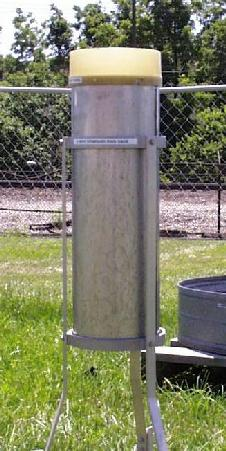
\includegraphics[width=\linewidth,height=0.55\textheight,keepaspectratio]{images/rain-gauge.jpg}
\end{column}
\begin{column}{0.54\textwidth}
\textbf{Rain gauges}

\vspace{2mm}
Collect precipitation at a location and measure its accumulated depth.

\vspace{4mm}
Direct point measurements, but sparse coverage between gauges.
\end{column}
\end{columns}
\vfill
{\tiny\color{gray}Photo: NOAA / National Weather Service.}
\note{Opening question: how would you measure rainfall just outside this building? A collector provides accumulation over a chosen interval. A gauge represents its location, not every point in a square kilometre. Exposure, wind, and instrument errors also matter. Photo reused from the existing defense deck.}
\end{frame}

\begin{frame}[t]
\slidetitle{Weather radar}
\begin{columns}[T]
\begin{column}{0.30\textwidth}
\centering
{\small\bfseries Scanning antenna}\par\vspace{1mm}
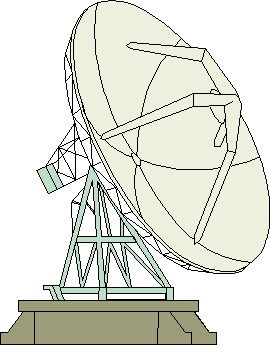
\includegraphics[width=\linewidth,height=0.36\textheight,keepaspectratio]{images/radar-antenna.png}
\figcredit{Source: FAA Aviation Weather Handbook, Chapter 15.}
\end{column}
\begin{column}{0.33\textwidth}
\centering
{\small\bfseries Transmitted pulse and echo}\par\vspace{1mm}
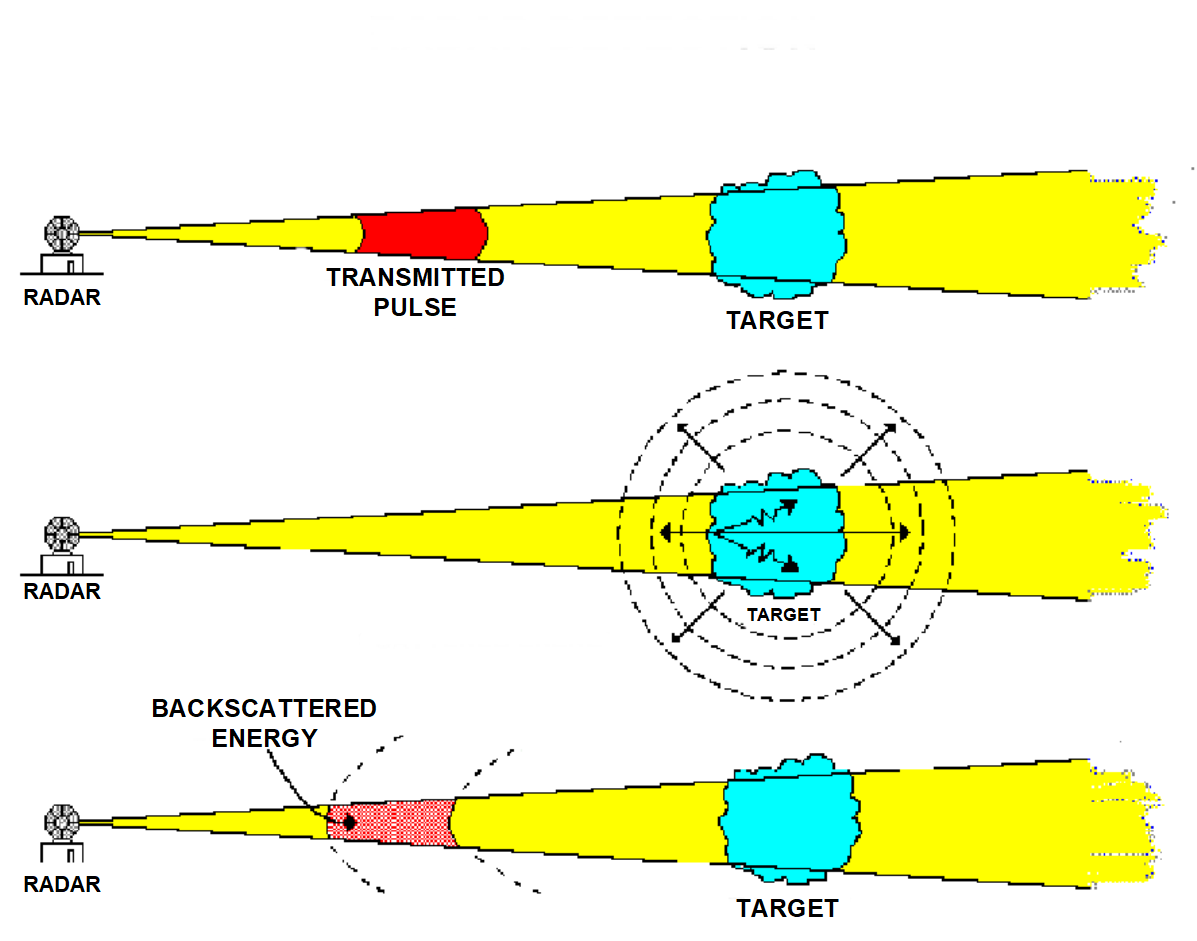
\includegraphics[width=\linewidth,height=0.32\textheight,keepaspectratio]{images/radar-backscatter.png}
\figcredit{Source: FAA Aviation Weather Handbook, Chapter 15.}
\end{column}
\begin{column}{0.33\textwidth}
\centering
{\small\bfseries Liquid-target reflectivity}\par\vspace{1mm}
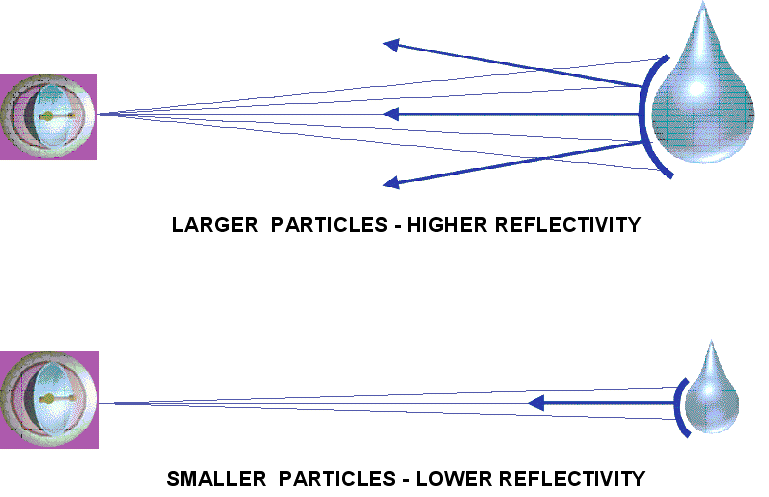
\includegraphics[width=\linewidth,height=0.32\textheight,keepaspectratio]{images/liquid-reflectivity.png}
\figcredit{Source: FAA Aviation Weather Handbook, Chapter 15.}
\end{column}
\end{columns}
\vspace{5mm}
\begin{itemize}
\item Reflectivity is converted into an estimated rain rate.
\item Broad spatial coverage, but the reflectivity-to-rain-rate conversion introduces uncertainty.
\end{itemize}
\vfill
\note{Figures from the FAA Aviation Weather Handbook, Chapter 15, reused from the existing defense deck. Explain the illustrations from left to right: the antenna scans and emits microwave pulses; raindrops scatter energy and a fraction returns as an echo; return delay locates the scattering volume, while corrected echo power supports an estimate of reflectivity. Drop-size distribution affects reflectivity and its conversion to rain rate. Reflectivity is not simply raw returned power. Radar offers broad spatial coverage, but rainfall retrieval introduces uncertainty.}
\end{frame}

\begin{frame}[t]
\slidetitle{Commercial microwave links in a cellular network}
\centering
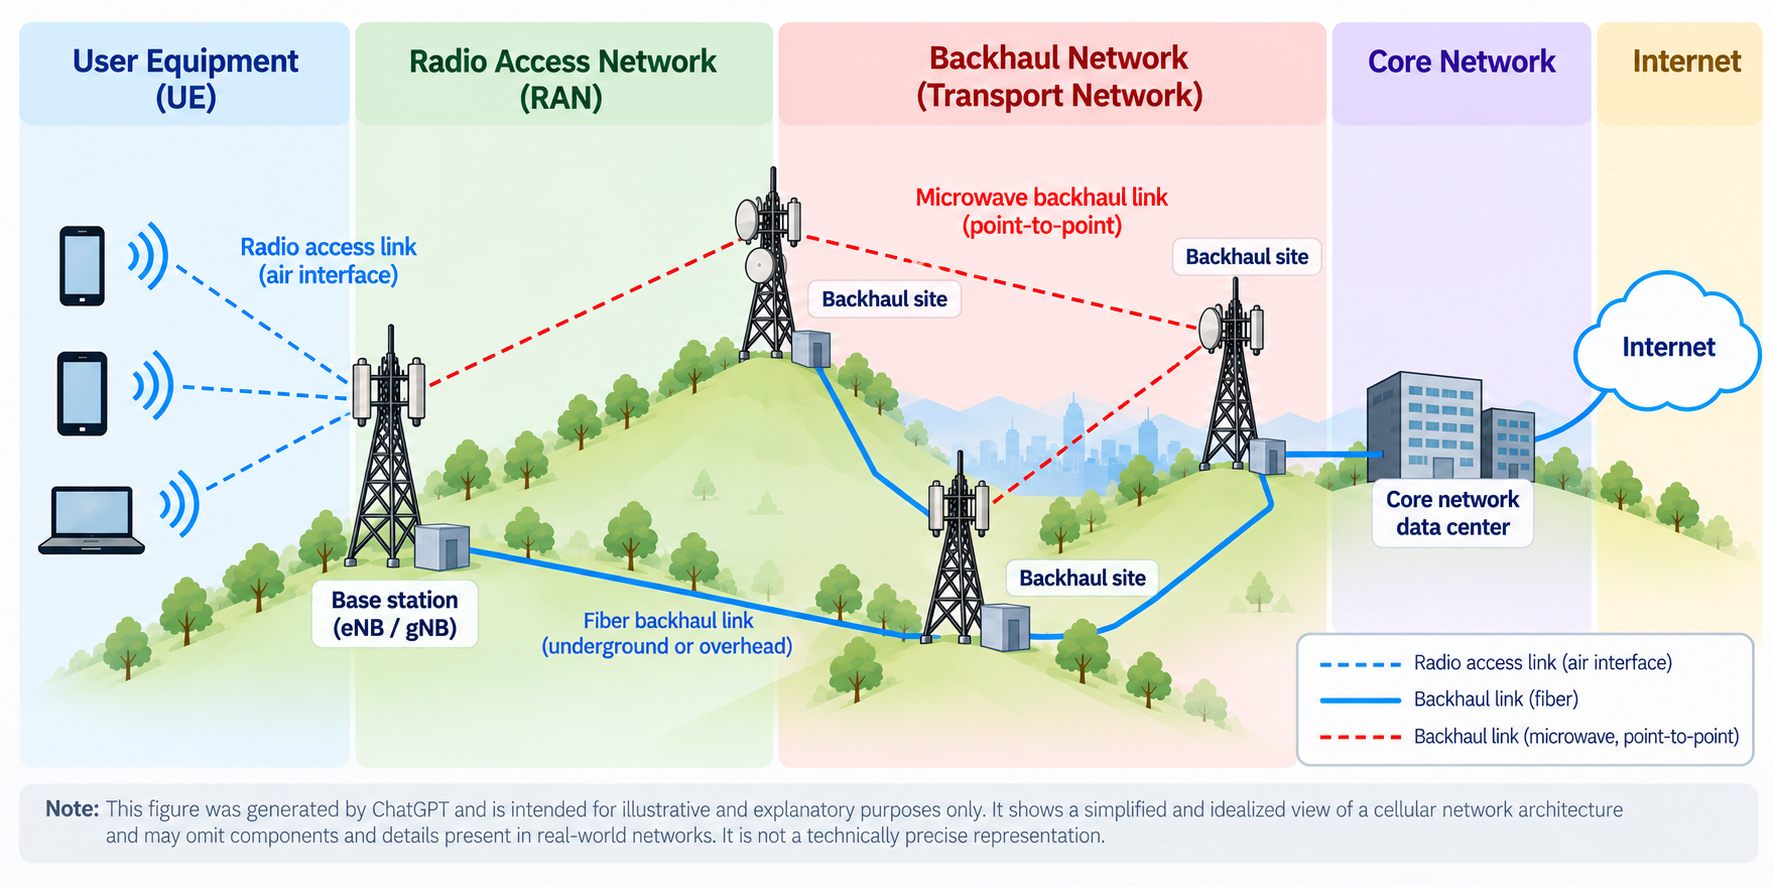
\includegraphics[width=0.98\textwidth,height=0.62\textheight,keepaspectratio]{images/cellular-network.png}
\par\vspace{2mm}
\small Red dashed connections: point-to-point microwave backhaul.\par
They carry users' communications.
\note{User-selected Cellular Network Architecture Infographic, an AI-generated schematic rather than a manufacturer diagram. Red dashed lines represent point-to-point microwave backhaul links. Blue dashed lines represent radio access, and solid blue lines represent fiber backhaul. Researchers use signal-level measurements on the microwave links, not the communications content.}
\end{frame}

\begin{frame}[t]
\slidetitle{Rain-induced attenuation}
\centering
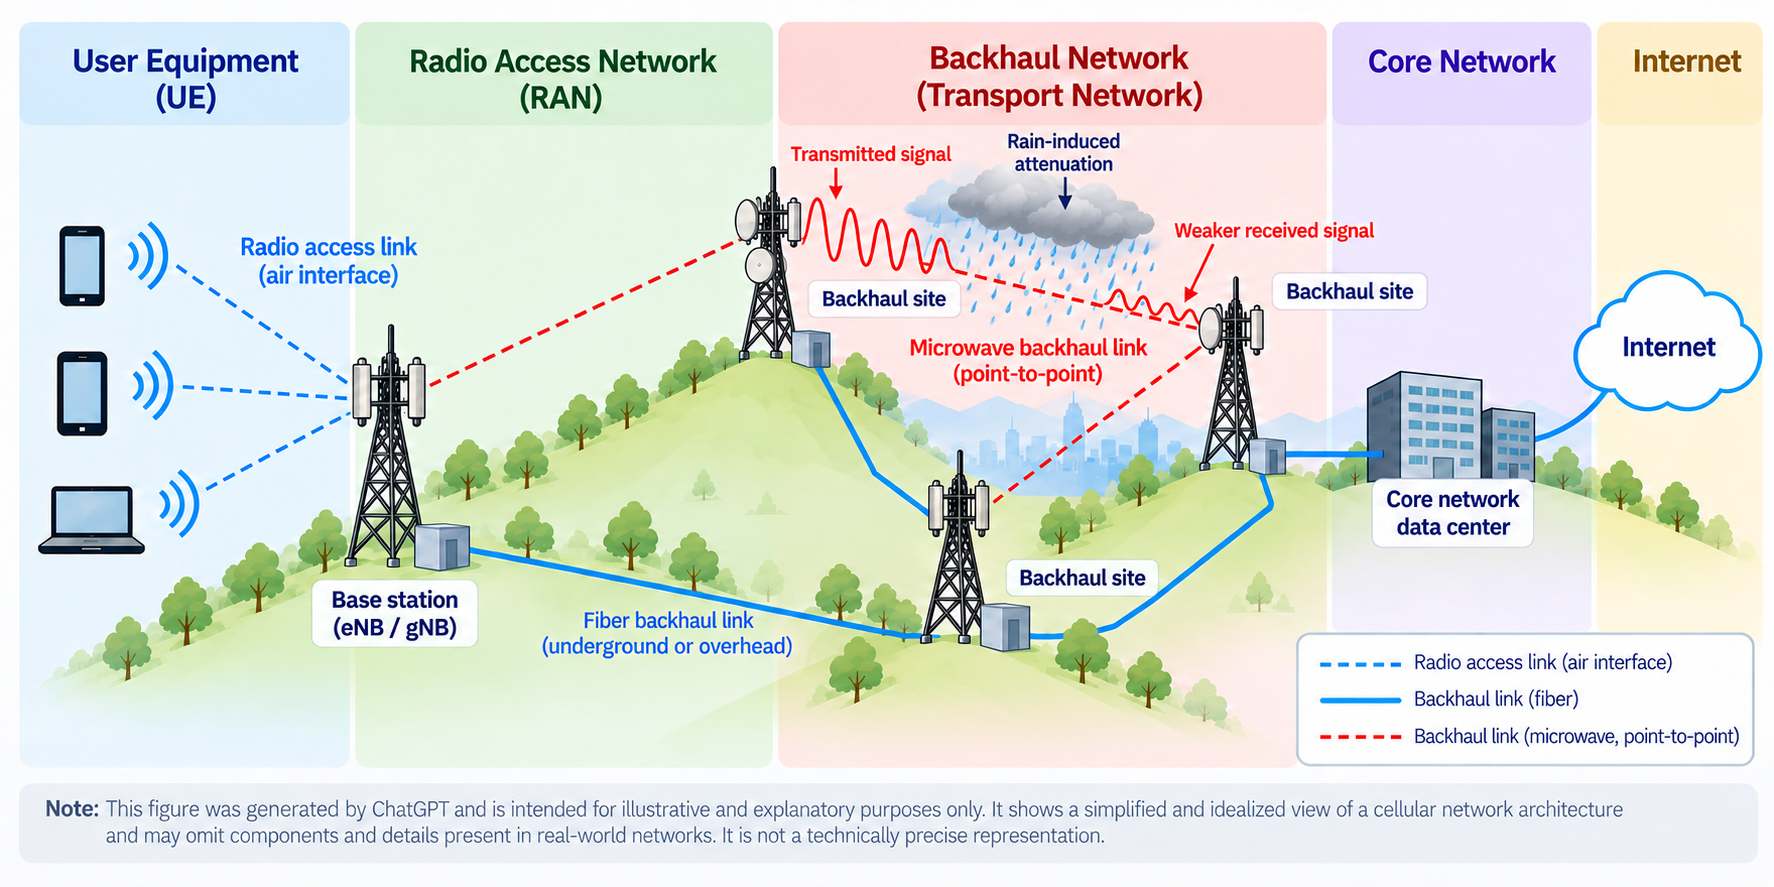
\includegraphics[width=0.98\textwidth,height=0.57\textheight,keepaspectratio]{images/cellular-network-rain-attenuation.png}
\par\vspace{2mm}
\begin{itemize}
\item When it rains, the microwave signal loses power.
\item This reduction in signal power along the link is called attenuation.
\item We use this signal loss to estimate rainfall along the link.
\end{itemize}
\note{AI-generated edit of the user-selected Cellular Network Architecture Infographic, not a manufacturer diagram. Rain crosses the upper microwave backhaul path. The decreasing wave amplitude schematically represents signal attenuation, not a cable, a changed carrier frequency, or a broken connection. The drawing is not to scale. Blue dashed access links connect devices to base stations. Backhaul transports aggregated traffic toward the core, using microwave or fiber. Rain sensing uses signal-level measurements rather than inspecting communication content. Edited asset: assets-v4/cellular-network-rain-attenuation.png.}
\end{frame}
% Earlier text-only version retained below for easy restoration.
\begin{comment}
\begin{frame}[t]
\frametitle{Glossary}
\textbf{Rain field} $R(s)$
\par\smallskip
A function from a rectangular geographic area $\Omega$ to non-negative real values:
\[R:\Omega\to\mathbb{R}_{\geq 0}.\]
For a pixel $s\in\Omega$, $R(s)$ is the rain rate at that pixel, measured in mm/h.

\vspace{2mm}
\textbf{Link} $\ell$
\begin{itemize}
\item A line segment between two geographic endpoints, specified by latitude and longitude.
\item Each link has a frequency $f_\ell$ and a polarization $p_\ell$.
\end{itemize}

\vspace{2mm}
\textbf{Specific attenuation} $\gamma_\ell(s)$
\begin{itemize}
\item Rain-induced signal loss per kilometre of link $\ell$ at location $s$ (dB/km).
\end{itemize}

\vspace{2mm}
\textbf{Total link attenuation} $A_\ell$
\begin{itemize}
\item The accumulated rain-induced signal loss along link $\ell$ (dB).
\end{itemize}
\note{A rain field assigns a nonnegative rain rate to each location in the area. Specific attenuation is local loss per unit path length; total link attenuation accumulates that loss along the link. Each considered link lies entirely within the area.}
\end{frame}
\end{comment}

\begin{frame}[t]
\frametitle{Glossary}
{\small\textbf{Link $\ell$:} a line segment joining two geographic endpoints (latitude and longitude), with frequency $f_\ell$ and polarization $p_\ell$.}
\vspace{1mm}
\begin{columns}[T,onlytextwidth]
\begin{column}{0.32\textwidth}
\centering
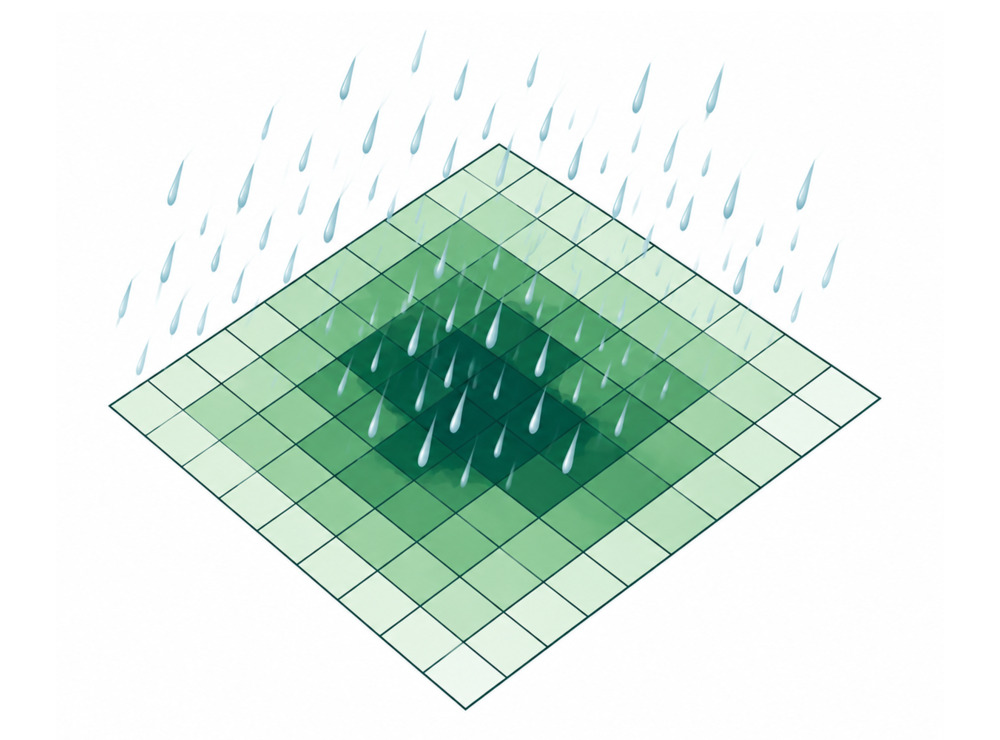
\includegraphics[width=\linewidth]{images/attenuation-sequence/01-rain-field-slide.jpg}\par\vspace{0.5mm}
{\tiny Conceptual illustration.}\par
{\footnotesize\textbf{Rain field $R(s)$}}\par
{\scriptsize $R:\Omega\to\mathbb{R}_{\geq 0}$. At pixel $s$, $R(s)$ is rain rate (mm/h).}
\end{column}
\begin{column}{0.32\textwidth}
\centering
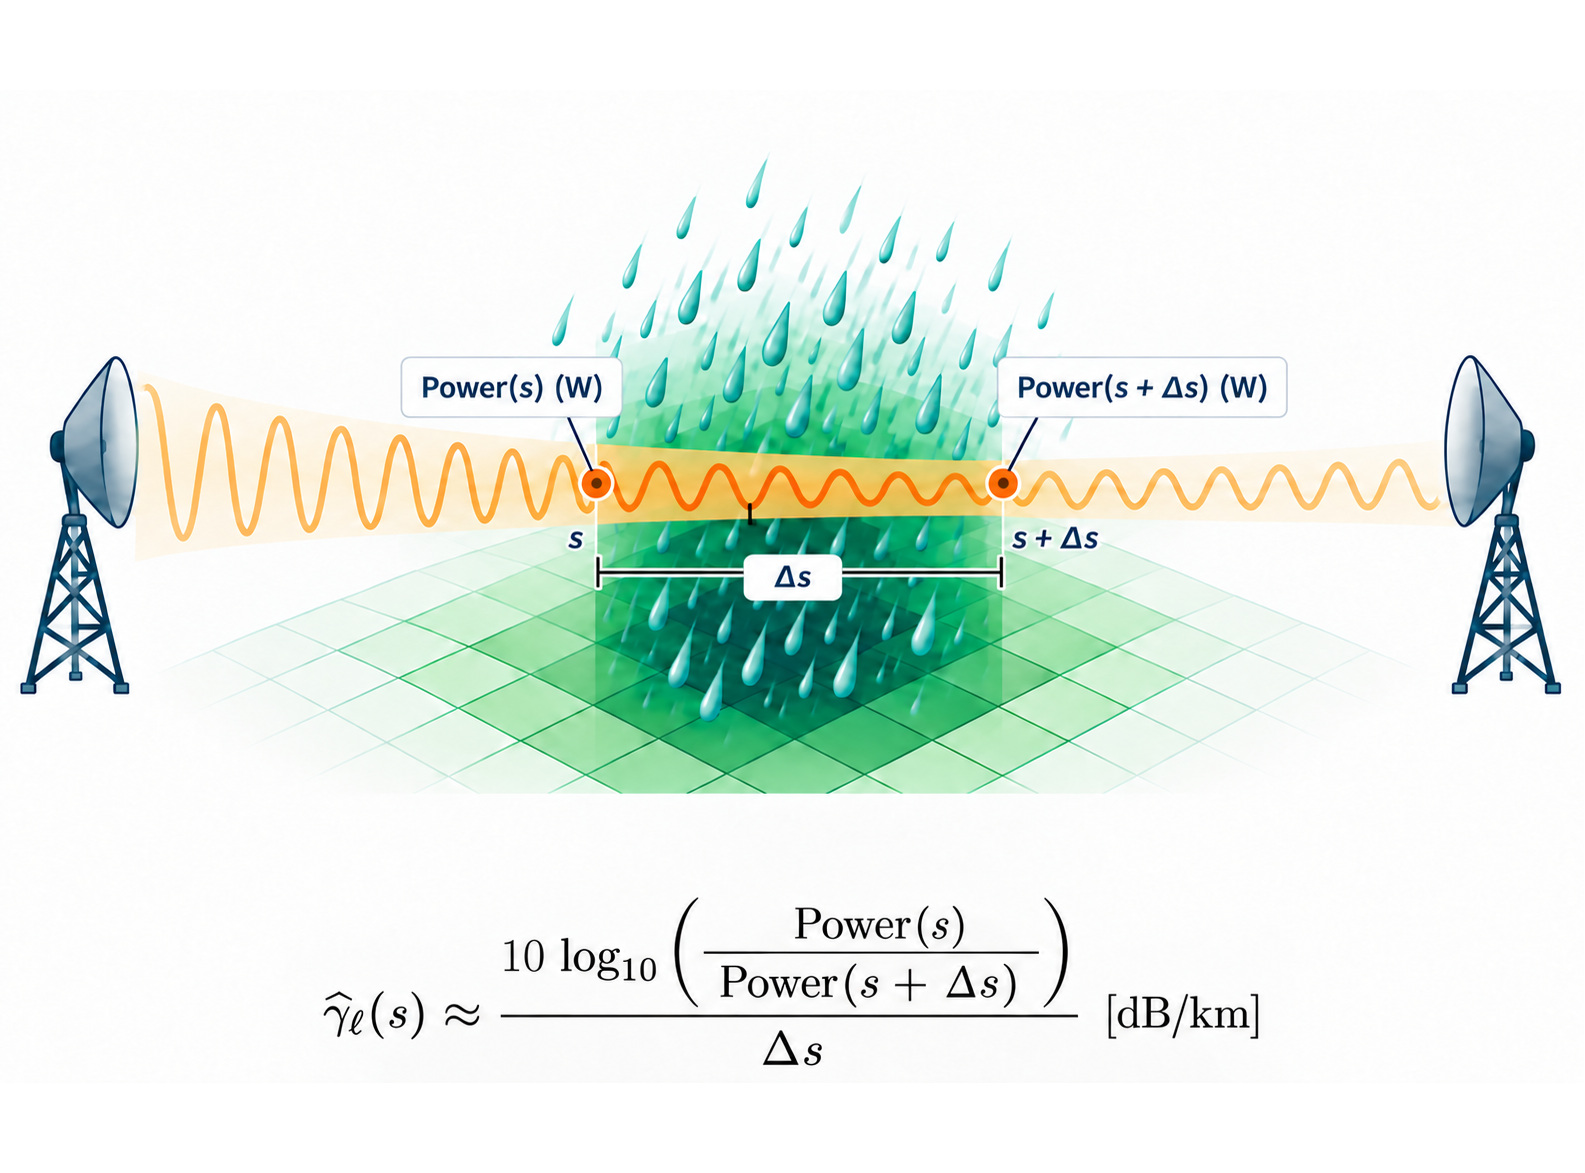
\includegraphics[width=\linewidth]{images/attenuation-sequence/02-specific-attenuation-slide-v4.jpg}\par\vspace{0.5mm}
{\tiny Conceptual illustration.}\par
{\footnotesize\textbf{Specific attenuation $\gamma_\ell(s)$}}\par
{\scriptsize Rain-induced signal loss per kilometre along link $\ell$ (dB/km).}
\end{column}
\begin{column}{0.32\textwidth}
\centering
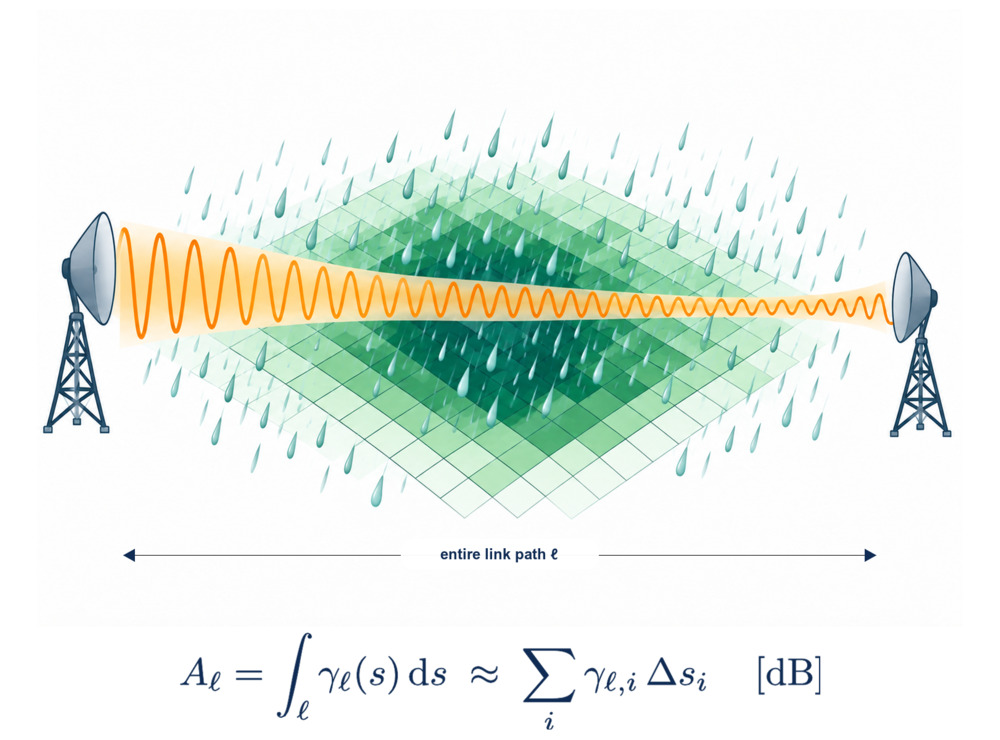
\includegraphics[width=\linewidth]{images/attenuation-sequence/03-total-attenuation-slide.jpg}\par\vspace{0.5mm}
{\tiny Conceptual illustration.}\par
{\footnotesize\textbf{Total attenuation $A_\ell$}}\par
{\scriptsize Accumulated rain-induced signal loss along the whole link (dB).}
\end{column}
\end{columns}
\note{The top line defines a link as a straight path between two geographic endpoints; each link also has frequency and polarization. The images connect the terms visually. Specific attenuation is local loss per unit path length. The middle graphic estimates $\gamma_\ell(s)$ from the measured power ratio over a one-kilometre segment. The ratio divided by segment length yields segment-mean specific attenuation; it approximates the local value when attenuation varies little across the segment. Total link attenuation integrates local specific attenuation over the full link. The modeled link paths lie entirely within $\Omega$.}
\end{frame}
\begin{frame}[t]
\frametitle{Problem Statement}
\textbf{We know:} an area $\Omega$ containing a set of links $\mathcal{L}$,
and their measured rain-induced attenuation $A_\ell$ for each link $\ell \in \mathcal{L}$.

\vspace{5mm}
\textbf{We want:} the unknown rainfall field across the area,
\[R:\Omega\to\mathbb R_{\geq 0},\qquad R(s)\text{ in mm/h}.\]

\vspace{3mm}
\textbf{Goal:} use the link paths and their attenuation measurements
to estimate the rainfall field $\widehat R$.
\note{This is the inverse problem in plain language. The modeled microwave-link paths lie entirely inside $\Omega$, so the full path is used in each attenuation integral. The observed quantity is rain-induced attenuation in dB; the target is a nonnegative rain-rate field over the area. We have not yet shown how a candidate field predicts attenuation—that is the forward model on the following slides.}
\end{frame}

\begin{comment}
\begin{frame}[t]
\frametitle{Link properties and specific attenuation}
Each microwave link has a \textbf{frequency} $f_\ell$ and
\textbf{polarization} $p_\ell$.

\vspace{3mm}
ITU-R Recommendation P.838-3 gives the rain-specific attenuation
for a local rain rate $R$:
\[\gamma_\ell(s)=\kappa(f_\ell,p_\ell)\,R(s)^{\alpha(f_\ell,p_\ell)}.\]

\vspace{2mm}
$\gamma_\ell$: signal loss per distance (dB/km)\qquad
$R$: rain rate (mm/h)
\vspace{4mm}
\begin{center}
{\small\textbf{Example ITU-R P.838-3 coefficients (horizontal polarization)}}\\[1mm]
\begin{tabular}{@{}rrr@{}}
\toprule
Frequency $f_\ell$ (GHz) & $\kappa$ & $\alpha$\\
\midrule
24.92  & 0.155896 & 0.999997\\
30.00  & 0.240308 & 0.948457\\
38.003 & 0.400172 & 0.881535\\
\bottomrule
\end{tabular}
\end{center}
\vspace{1mm}
{\scriptsize Illustrative frequencies; coefficients depend on frequency and polarization.}
\note{ITU-R is the International Telecommunication Union's radiocommunication sector. Recommendation P.838-3 specifies coefficients for the power-law relation between rain rate and specific attenuation as a function of frequency and polarization. The table values were evaluated from the project's P.838-3 implementation for horizontal polarization at zero elevation; they are illustrative examples, not a claim about every link in the dataset. Specific attenuation is local loss per unit path length. Integrating it along a link gives rain-induced link attenuation, which is the forward model on the next slide.}
\end{frame}
\end{comment}


\begin{frame}[t]
\slidetitle{The rainfall-to-attenuation model}
\centering
{\small\raggedright ITU-R P.838-3 maps local rain rate to rain-induced loss per unit distance.\par}
\vspace{-2mm}
\[
\gamma_\ell(s)=\kappa(f_\ell,p_\ell)\,R(s)^{\alpha(f_\ell,p_\ell)}.
\]
\small $R(s)$ in mm/h; $\gamma_\ell(s)$ in dB/km.\par
\vspace{1mm}
{\small\textbf{Example coefficients (horizontal polarization)}}\par
\vspace{1mm}
{\renewcommand{\arraystretch}{1.2}
\setlength{\tabcolsep}{12pt}
\begin{tabular}{@{}rcc@{}}
\toprule
\rowcolor{MutedBlue}\textbf{Frequency $f_\ell$ (GHz)} & $\boldsymbol{\kappa}$ & $\boldsymbol{\alpha}$\\
\midrule
\rowcolor{MutedBlue}24.92  & 0.155896 & 0.999997\\
30.00  & 0.240308 & 0.948457\\
\rowcolor{MutedBlue}38.003 & 0.400172 & 0.881535\\
\bottomrule
\end{tabular}}

\vspace{2mm}
{\small\raggedright\textbf{Integrate along a link to obtain total attenuation:}\par}\vspace{-2mm}
\[
\widehat A_\ell(R)=\int_\ell\gamma_\ell(s)\,\mathrm ds
\qquad [\mathrm{dB}].
\]
\vspace{1mm}
{\tiny Coefficient model: ITU-R Recommendation P.838-3 (2005).}
\note{This is the forward construction: ITU-R P.838-3 converts local rain rate to specific attenuation, with coefficients depending on frequency and polarization. The table values were evaluated from the project's P.838-3 implementation for horizontal polarization at zero elevation; they are examples, not a claim about every link in the dataset. Integrating specific attenuation along the full modeled link gives predicted rain-induced attenuation in dB. The path integral is discretized over pixels in the computational formulation.}
\end{frame}

\begin{frame}[t]
\slidetitle{Milestones in microwave rainfall sensing}
\small
\renewcommand{\arraystretch}{1.3}
\setlength{\tabcolsep}{2pt}
\begin{tabular}{@{}p{0.16\textwidth}p{0.79\textwidth}@{}}
\textbf{1946--1954} & \textbf{J. W. Ryde; Gunn \& East}\newline
Ryde noted near-linearity ($\alpha=1$); Gunn \& East proposed $\gamma_R=kR^\alpha$.\\
\textbf{1977--1978} & \textbf{Atlas \& Ulbrich; Olsen et al.}\newline
Physical basis: near-linearity at selected frequencies and power-law models.\\
\textbf{1991} & \textbf{Giuli et al.}\newline
Tomographic rainfall-field reconstruction from simulated link attenuations.\\
\textbf{2000--2003} & \textbf{Holt et al.; Rahimi et al.}\newline
Dedicated dual-frequency links: path rainfall compared with gauges and radar.\\
\textbf{2006--2007} & \textbf{Messer et al.; Leijnse et al.}\newline
Rainfall retrieval from commercial links in Israel and the Netherlands.\\
\textbf{2013 / 2016} & \textbf{Overeem et al.}\newline
Netherlands-wide maps using ordinary kriging; later, 2.5 years of maps.\\
\textbf{2020} & \textbf{Graf et al.}\newline
German-wide evaluation with approximately 4,000 CMLs and IDW.\\
\end{tabular}
\par\vspace{0mm}
Our comparison uses IDW, an established baseline in large-scale CML rainfall mapping.
\note{Optional background slide, retained from version 13. These are selected milestones, not a complete history. The distinction here is that Ryde's early Mie calculations pointed to an approximate linear form ($\alpha=1$), while Gunn and East's 1954 treatment developed a more general power-law description. These are historical approximations, not universal exponents; the fitted exponent depends on frequency and rain microphysics. Avoid claiming Ryde alone made the first observation of the rain-rate/attenuation relationship: contemporaneous empirical studies also appeared in 1946. Dedicated experimental links are distinct from opportunistic sensing with an existing commercial network. Atlas and Ulbrich demonstrated near-linearity under selected frequency and microphysical conditions, not a universal linear relationship. Olsen and colleagues assessed power-law approximations using Mie calculations and experimental comparisons; their tables should not be equated with modern polarization-dependent ITU coefficients. Giuli used simulated observations and recursive tomographic reconstruction; the exact objective and common-frequency assumptions remain unverified. Rahimi et al. (2003) used an approximately linear relation between dual-frequency attenuation differences and path-average rainfall, not simply direct Olsen inversion. Messer (2006) and Leijnse (2007) demonstrated commercial-link rainfall retrieval rather than a validated nationwide mapping product. Overeem (2013) used approximately 2,400 links; the 2016 study produced 15-minute maps over 2.5 years using an average of 3,383 directional links on 2,044 paths. Graf (2020) used approximately 4,000 German links and IDW. IDW and kriging predate these studies. Sources: Ryde, doi:10.1049/JI-3A-1.1946.0029; Gunn and East, doi:10.1002/qj.49708034603; historical account in NASA NTRS Report 19740006157; Atlas and Ulbrich, doi:10.1175/1520-0450(1977)016<1322:PAAIRM>2.0.CO;2; Olsen et al., doi:10.1109/TAP.1978.1141845; Giuli et al., doi:10.1175/1520-0450(1991)030<1323:TRORFT>2.0.CO;2; Rahimi et al., doi:10.1029/2002JD003202; Messer et al., doi:10.1126/science.1120034; Leijnse et al., doi:10.1029/2006WR005631; Overeem et al., doi:10.1073/pnas.1217961110 and doi:10.1002/2016WR019412; Graf et al., https://hess.copernicus.org/articles/24/2931/2020/.}
\end{frame}

\begin{comment}
\begin{frame}[t]
\slidetitle{The rain-attenuation forward model}
\textbf{Specific attenuation}
\[\gamma_\ell(R)=\kappa_\ell R^{\alpha_\ell}\qquad[\mathrm{dB/km}].\]
\textbf{Attenuation along a link}
\[A_\ell(R)=\int_\ell\kappa_\ell R(s)^{\alpha_\ell}\,ds
=\sum_{p\in\mathcal C(\ell)}d_{\ell,p}\kappa_\ell R_p^{\alpha_\ell}.\]
\vspace{2mm}
$d_{\ell,p}$: crossed length in pixel $p$, in km.\par
$R_p$: rain rate in mm/h.\par
Frequency and polarization determine $\kappa_\ell$ and $\alpha_\ell$.
\note{ITU-R P.838-3 power law. The discrete expression assumes a constant rain rate within each computational pixel. Attenuation is rain-induced loss in dB, distinguished from total path loss. Inverting average specific attenuation gives a uniform rain equivalent, not generally the arithmetic path-average rainfall.}
\end{frame}

\begin{frame}[t]
\slidetitle{Unknown rain field, measured link attenuation}
\centering
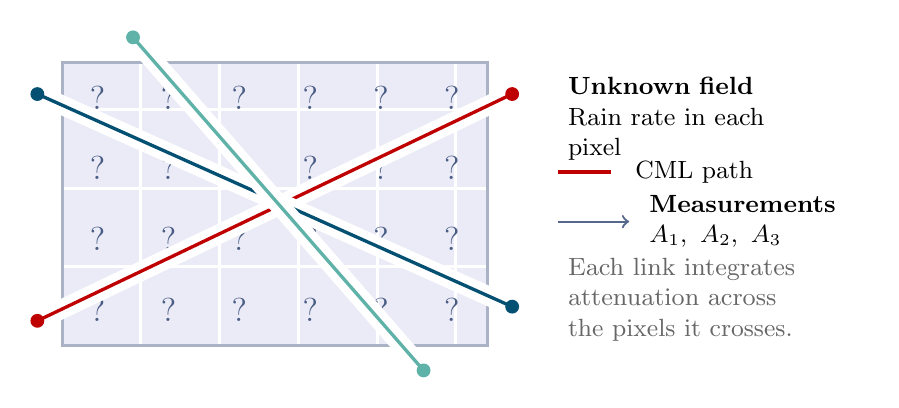
\begin{tikzpicture}[x=0.9cm,y=0.9cm, every node/.style={font=\small}]
  % A calm, large grid: each question mark is one unknown pixel value.
  \fill[MutedBlue] (0,0) rectangle (6,4);
  \draw[white,line width=1.1pt] (0,0) grid (6,4);
  \draw[DarkBlue!35,line width=1pt] (0,0) rectangle (6,4);
  \foreach \x in {0.5,1.5,2.5,3.5,4.5,5.5}
    \foreach \y in {0.5,1.5,2.5,3.5}
      \node[text=DarkBlue!75,font=\large] at (\x,\y) {?};

  % Link paths sit visibly over the pixel grid.
  \draw[white,line width=7pt] (-0.35,0.35)--(6.35,3.55);
  \draw[very thick,red!75!black] (-0.35,0.35)--(6.35,3.55);
  \draw[white,line width=7pt] (-0.35,3.55)--(6.35,0.55);
  \draw[very thick,MediumBlue] (-0.35,3.55)--(6.35,0.55);
  \draw[white,line width=7pt] (1.0,4.35)--(5.1,-0.35);
  \draw[very thick,MediumGreen] (1.0,4.35)--(5.1,-0.35);
  \foreach \x/\y/\c in {
    -0.35/0.35/red!75!black,6.35/3.55/red!75!black,
    -0.35/3.55/MediumBlue,6.35/0.55/MediumBlue,
    1.0/4.35/MediumGreen,5.1/-0.35/MediumGreen}
    \fill[\c] (\x,\y) circle (2.5pt);

  % Legend and corresponding path-integrated measurements.
  \node[anchor=west,align=left,text width=3.15cm] at (7.0,3.2)
    {\textbf{Unknown field}\\Rain rate in each pixel};
  \draw[very thick,red!75!black] (7.0,2.45)--(7.75,2.45);
  \node[anchor=west] at (7.95,2.45) {CML path};
  \draw[->,thick,DarkBlue!70] (7.0,1.75)--(8.0,1.75);
  \node[anchor=west,align=left,text width=2.7cm] at (8.15,1.75)
    {\textbf{Measurements}\\$A_1,\ A_2,\ A_3$};
  \node[anchor=west,align=left,text width=3.1cm,text=gray!80!black] at (7.0,0.65)
    {Each link integrates attenuation across the pixels it crosses.};
\end{tikzpicture}
\note{Conceptual diagram, not to scale. Each question mark represents an unknown rain-rate value in one pixel. Colored line segments represent microwave links crossing multiple pixels. Each link provides one path-integrated attenuation measurement. The forward model predicts these measurements from a candidate rain field; the inverse problem uses the measurements to estimate that field.}
\end{frame}
\end{comment}

% Previous benchmark-slide layout retained for easy restoration.
% Uncomment this frame and comment out the new pipeline frame below to return to it.
\begin{comment}
\begin{frame}[t]
\slidetitle{Methodology}
\begin{columns}[c]
\begin{column}{0.56\textwidth}
\deckimage[width=\linewidth,height=0.59\textheight,keepaspectratio]{images/benchmark-patches.png}{100 benchmark patch locations}
\end{column}
\begin{column}{0.4\textwidth}
\textbf{100 precipitation patches}\par
\vspace{2mm}
84 hourly EURADCLIM maps\par
18--31 January 2023\par
Native grid: $2\times2$ km\par
\vspace{3mm}
4TU Netherlands network template\par
939--1,996 observations per patch
\end{column}
\end{columns}
\note{Source: thesis and existing benchmark slide. EURADCLIM combines OPERA radar precipitation and gauge information. Network geometry and frequencies provide the template, not operational received-power observations. Multiple frequencies on a path count as separate observations. Event-selected patches are not a random sample of European weather.}
\end{frame}
\end{comment}

\begin{frame}[t]
\slidetitle{Benchmark construction}
\centering
{\small\color{black!65}From European precipitation maps to synthetic link observations}\par\vspace{4mm}
\begin{tikzpicture}[x=1cm,y=1cm,>=stealth,
  stage/.style={draw=DarkBlue!22,rounded corners=2.5mm,fill=white,
    line width=.8pt,minimum width=2.9cm,minimum height=4.75cm,
    align=center,inner sep=2.5mm},
  stagetitle/.style={font=\small\bfseries,text=DarkBlue,align=center},
  detail/.style={font=\scriptsize,align=center,text=black!78},
  flow/.style={->,line width=1.25pt,draw=MediumBlue},
  badge/.style={circle,fill=MediumBlue,text=white,font=\scriptsize\bfseries,
    inner sep=1.3pt,minimum size=5mm}]
\node[stage] (data) at (1.45,0) {};
\node[badge] at (data.north east) [xshift=-2mm,yshift=-2mm] {1};
\node[stagetitle] at (data.center) [yshift=16mm] {Precipitation fields};
% EURADCLIM V3 precipitation map; the data source is credited below.
\node at (data.center) [yshift=0.5mm]
  {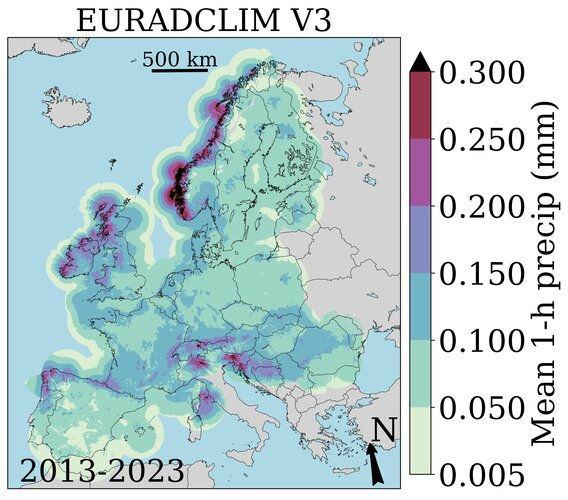
\includegraphics[width=2.4cm,height=1.65cm,keepaspectratio]{images/benchmark-euradclim.jpg}};
\node[detail,text width=2.65cm] at (data.center) [yshift=-13mm]
  {84 hourly maps\\18--31 Jan 2023\\2 km grid};
\node[font=\tiny,align=center,text=black!65] at (data.center) [yshift=-21.5mm]
  {KNMI / EURADCLIM};

\node[stage] (patches) at (4.65,0) {};
\node[badge] at (patches.north east) [xshift=-2mm,yshift=-2mm] {2};
\node[stagetitle] at (patches.center) [yshift=16mm] {Patch selection};
\node at (patches.center) [yshift=0.5mm]
  {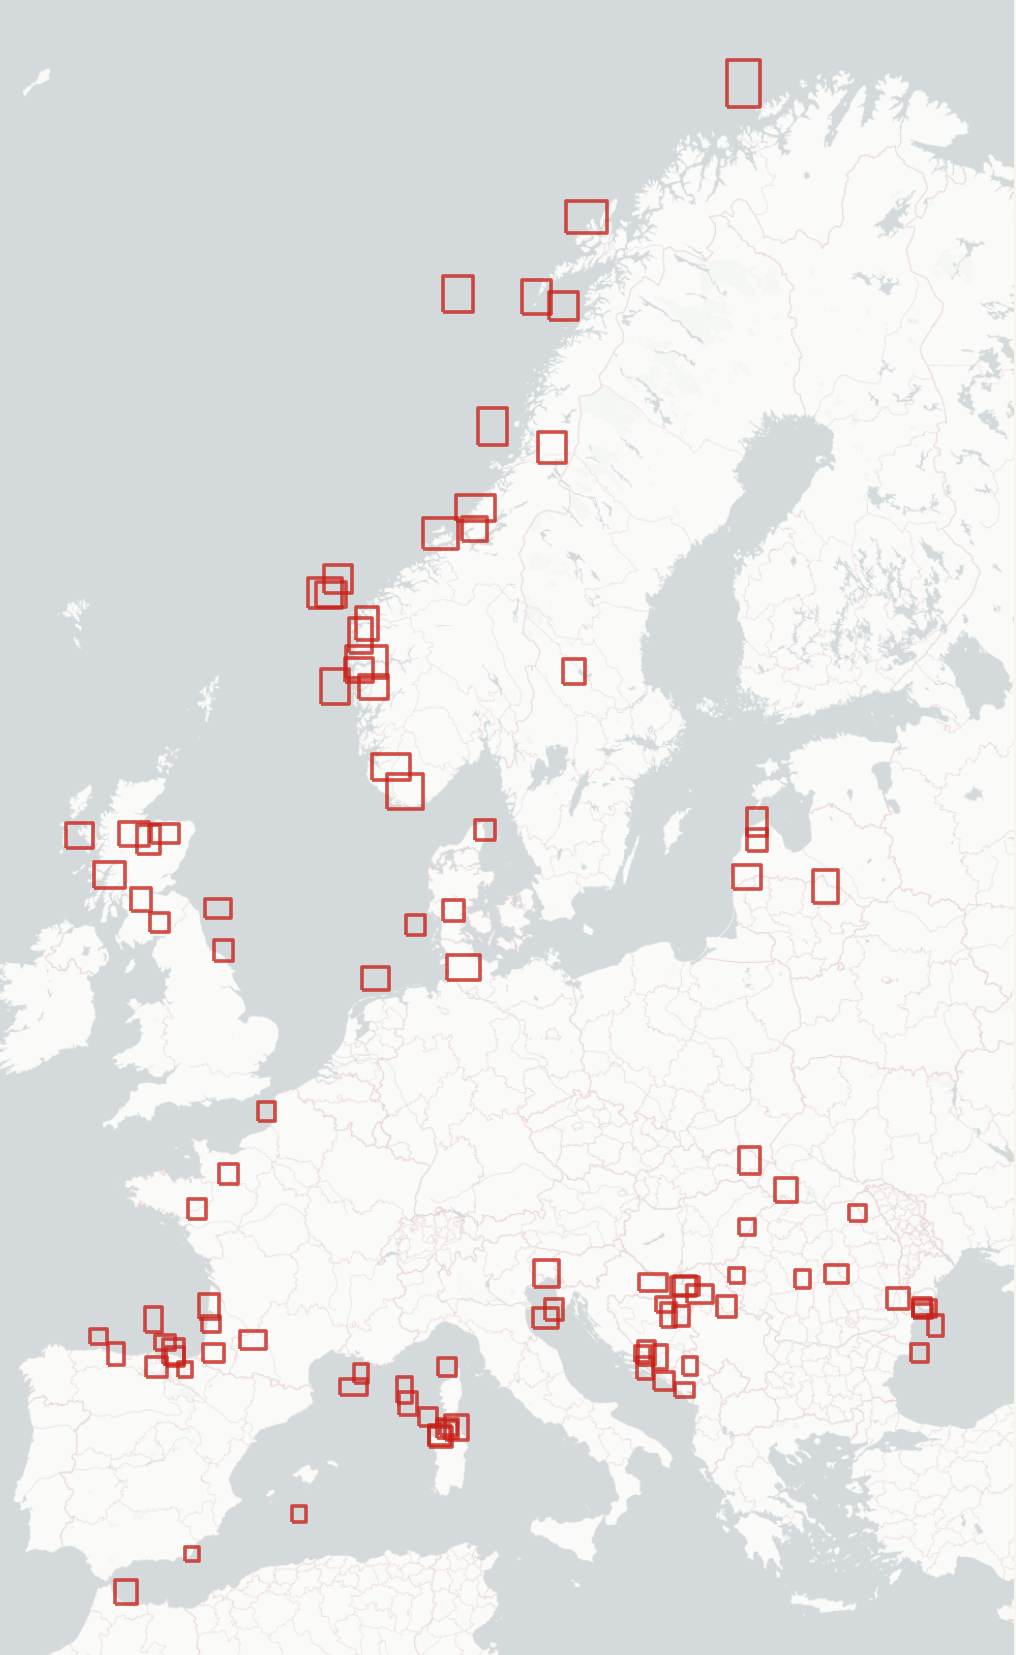
\includegraphics[height=1.65cm,width=2.4cm,keepaspectratio]{images/benchmark-100-patch-locations.png}};
\node[detail,text width=2.65cm] at (patches.center) [yshift=-13mm]
  {Detect rain events;\\select \textbf{100 patches}};
\node[font=\tiny,align=center,text=black!65] at (patches.center) [yshift=-21.5mm]
  {Basemap: OSM / CARTO};

\node[stage] (links) at (7.85,0) {};
\node[badge] at (links.north east) [xshift=-2mm,yshift=-2mm] {3};
\node[stagetitle] at (links.center) [yshift=16mm] {Network template};
% Netherlands CML network map, cropped to the map area.
\node at (links.center) [yshift=0.5mm]
  {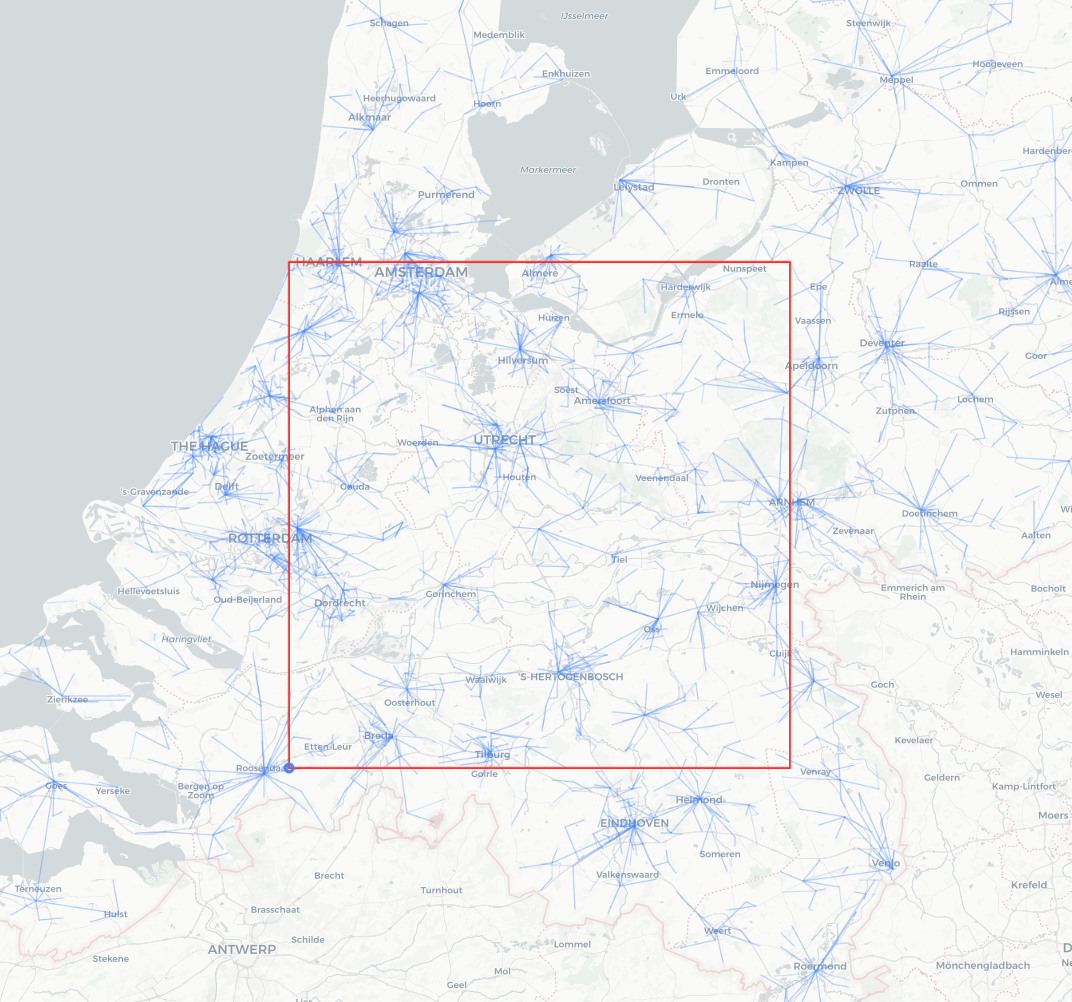
\includegraphics[width=2.4cm,height=1.65cm,keepaspectratio,
    trim={248bp 194bp 242bp 223bp},clip]{images/benchmark-4tu-network.png}};
\node[detail,text width=2.65cm] at (links.center) [yshift=-13mm]
  {4TU Netherlands\\Mean: \textbf{1,324 per patch}\\Range: 939--1,996};
\node[font=\tiny,align=center,text=black!65] at (links.center) [yshift=-21.5mm]
  {4TU data + OSM / CARTO};

\node[stage] (clip) at (11.05,0) {};
\node[badge] at (clip.north east) [xshift=-2mm,yshift=-2mm] {4};
\node[stagetitle] at (clip.center) [yshift=16mm] {Synthetic link data};
% EURADCLIM rainfall crop with author-overlaid 4TU CML geometry.
\node at (clip.center) [yshift=0.5mm]
  {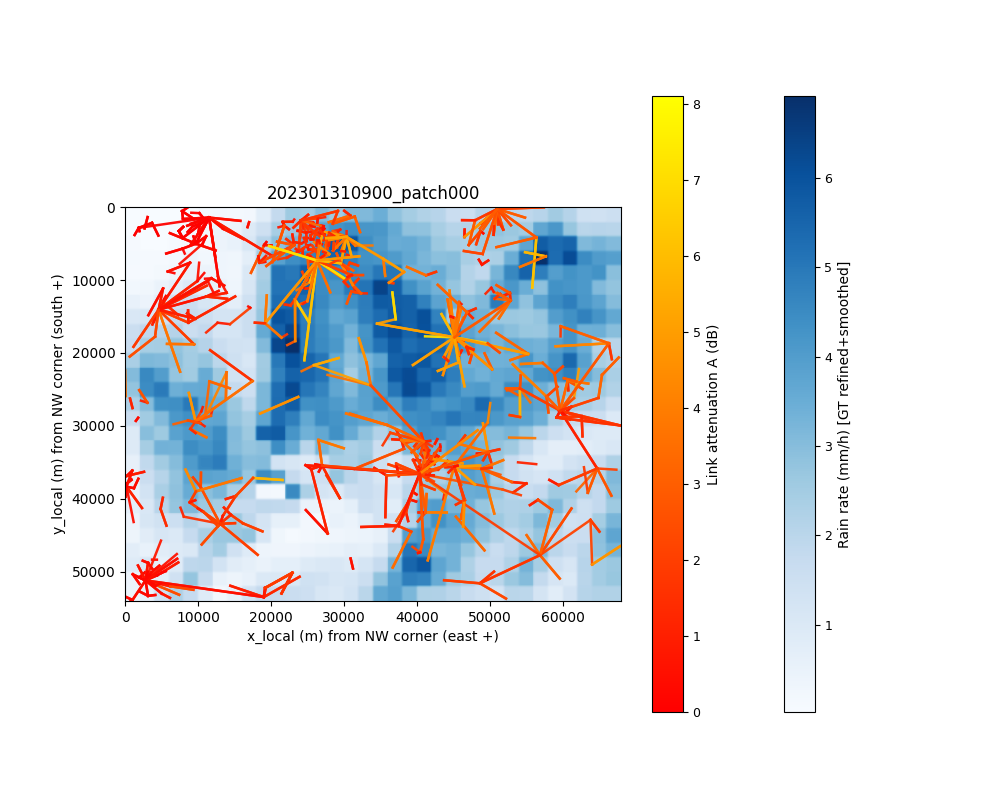
\includegraphics[width=2.4cm,height=1.65cm,keepaspectratio,
    trim={95bp 68bp 282bp 155bp},clip]{images/benchmark-example-overlay.png}};
\node[detail,text width=2.65cm] at (clip.center) [yshift=-13mm]
  {Clip link paths to the patch\\Simulate rain-induced attenuation};
\node[font=\tiny,align=center,text=black!65] at (clip.center) [yshift=-21.5mm]
  {EURADCLIM + 4TU links};

\draw[flow] (data.east)--(patches.west);
\draw[flow] (patches.east)--(links.west);
\draw[flow] (links.east)--(clip.west);
\end{tikzpicture}
\par\vspace{1mm}
\colorbox{MutedBlue}{\parbox{.93\linewidth}{\centering\scriptsize
We use the 4TU link geometry and frequencies, but not the received signal levels (RSLs). Attenuation is simulated from each reference rainfall field.}}
\note{Explain the pipeline left to right. EURADCLIM supplies 84 hourly precipitation maps from 18--31 January 2023 at a native 2 km grid. The first image is the EURADCLIM V3 mean one-hour precipitation map, shown as dataset context rather than as one of the 84 benchmark frames. A detector identifies precipitation patches; 100 are selected, and their European distribution is mapped over OpenStreetMap data with CARTO basemap tiles. We use link geometry and carrier frequencies from the 4TU Netherlands dataset. Its network overview uses the same OpenStreetMap/CARTO basemap. For each selected patch, only links whose two endpoints fall inside the patch are retained. This gives 939--1,996 link observations per patch, with a mean of 1,324; each frequency on a physical path counts as a separate observation. We do not use the received signal levels (RSLs); instead, we simulate attenuation from each reference rainfall field. The example overlay combines an EURADCLIM rainfall patch with retained 4TU link geometry, clipped and overlaid by the author. Full data sources: Overeem et al. (2023, 2025) for EURADCLIM and Overeem et al. (2024) for the 4TU dataset. EURADCLIM combines OPERA radar precipitation and gauge information. Event-selected patches are not a random sample of European weather.}
\end{frame}

\begin{frame}[t]
\slidetitle{Example benchmark patches}
\begin{columns}[c,onlytextwidth]
\begin{column}{.55\textwidth}
\centering
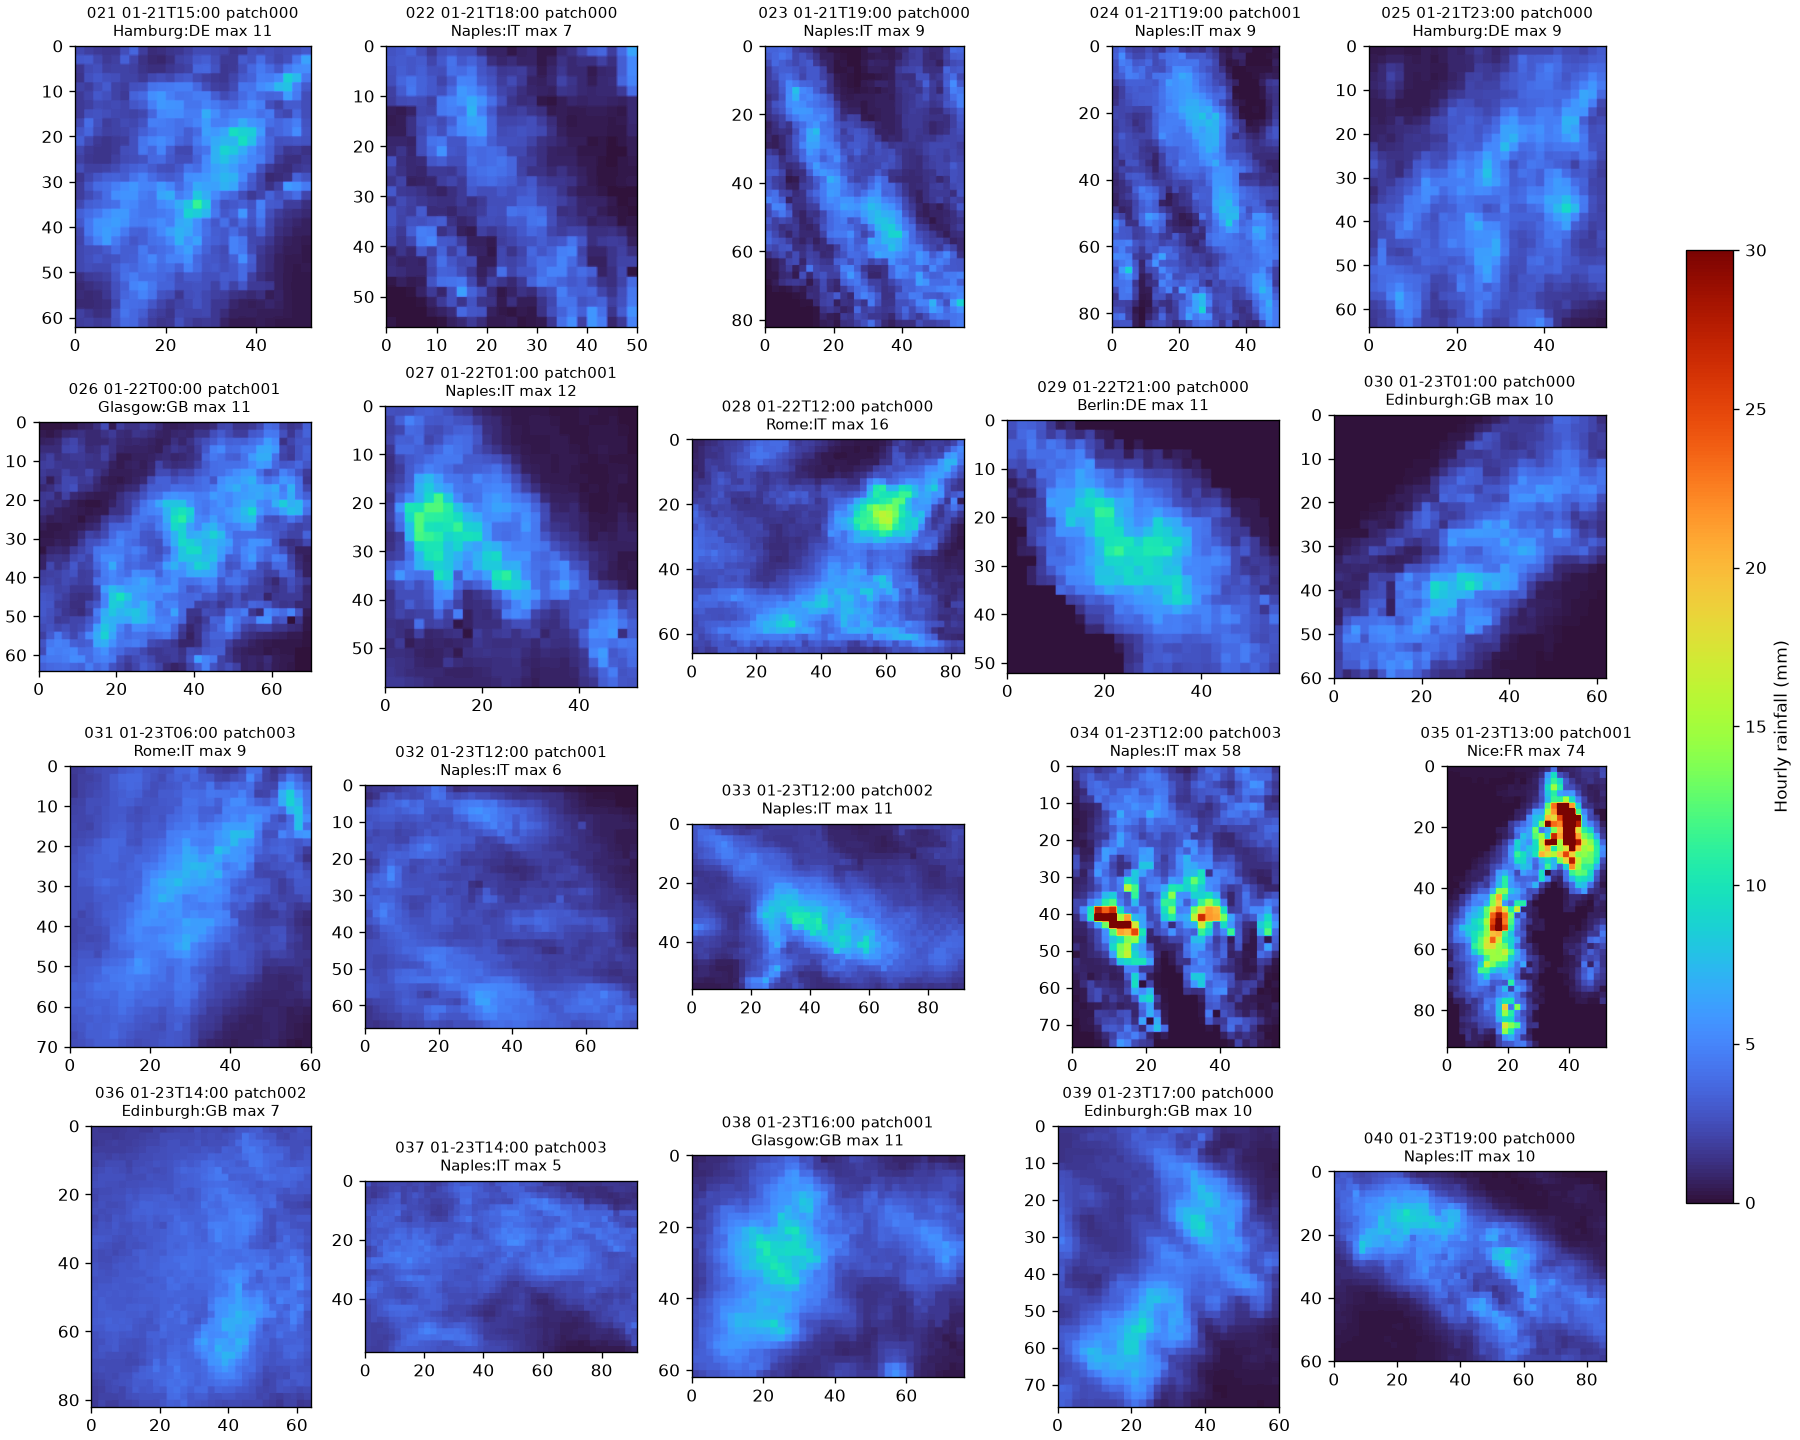
\includegraphics[width=\linewidth,height=.70\textheight,keepaspectratio]{images/benchmark-patch-examples.png}
\par\vspace{1mm}
{\tiny Examples of benchmark rainfall patches from EURADCLIM.}
\end{column}
\begin{column}{.41\textwidth}
\small
Each panel shows one selected hourly rainfall patch. The color scale is hourly rainfall accumulation (mm); the axes show native grid-cell indices.\par\medskip
The 100-patch benchmark samples 84 hourly EURADCLIM maps from 18--31 January 2023. The source maps have a 2 km grid.\par\medskip
These examples show the range of patch shapes and rainfall patterns used to simulate link attenuations.
\end{column}
\end{columns}
\note{The contact sheet is the user-specified review-02.png from Compute-Link-Attenuations/HundredPatches/review-sheets. It contains selected EURADCLIM-derived patches, not a representative or random sample. The local city/date labels and per-patch maxima were already present in that project review sheet; the color bar shows hourly rainfall accumulation in millimetres. The benchmark uses 100 patches from 84 hourly maps between 18 and 31 January 2023 at 2 km native resolution.}
\end{frame}

\begin{frame}[t]
\slidetitle{Patch geometry and link distributions}
\begin{columns}[T,onlytextwidth]
\begin{column}{.34\textwidth}
\centering
\vspace{0pt}
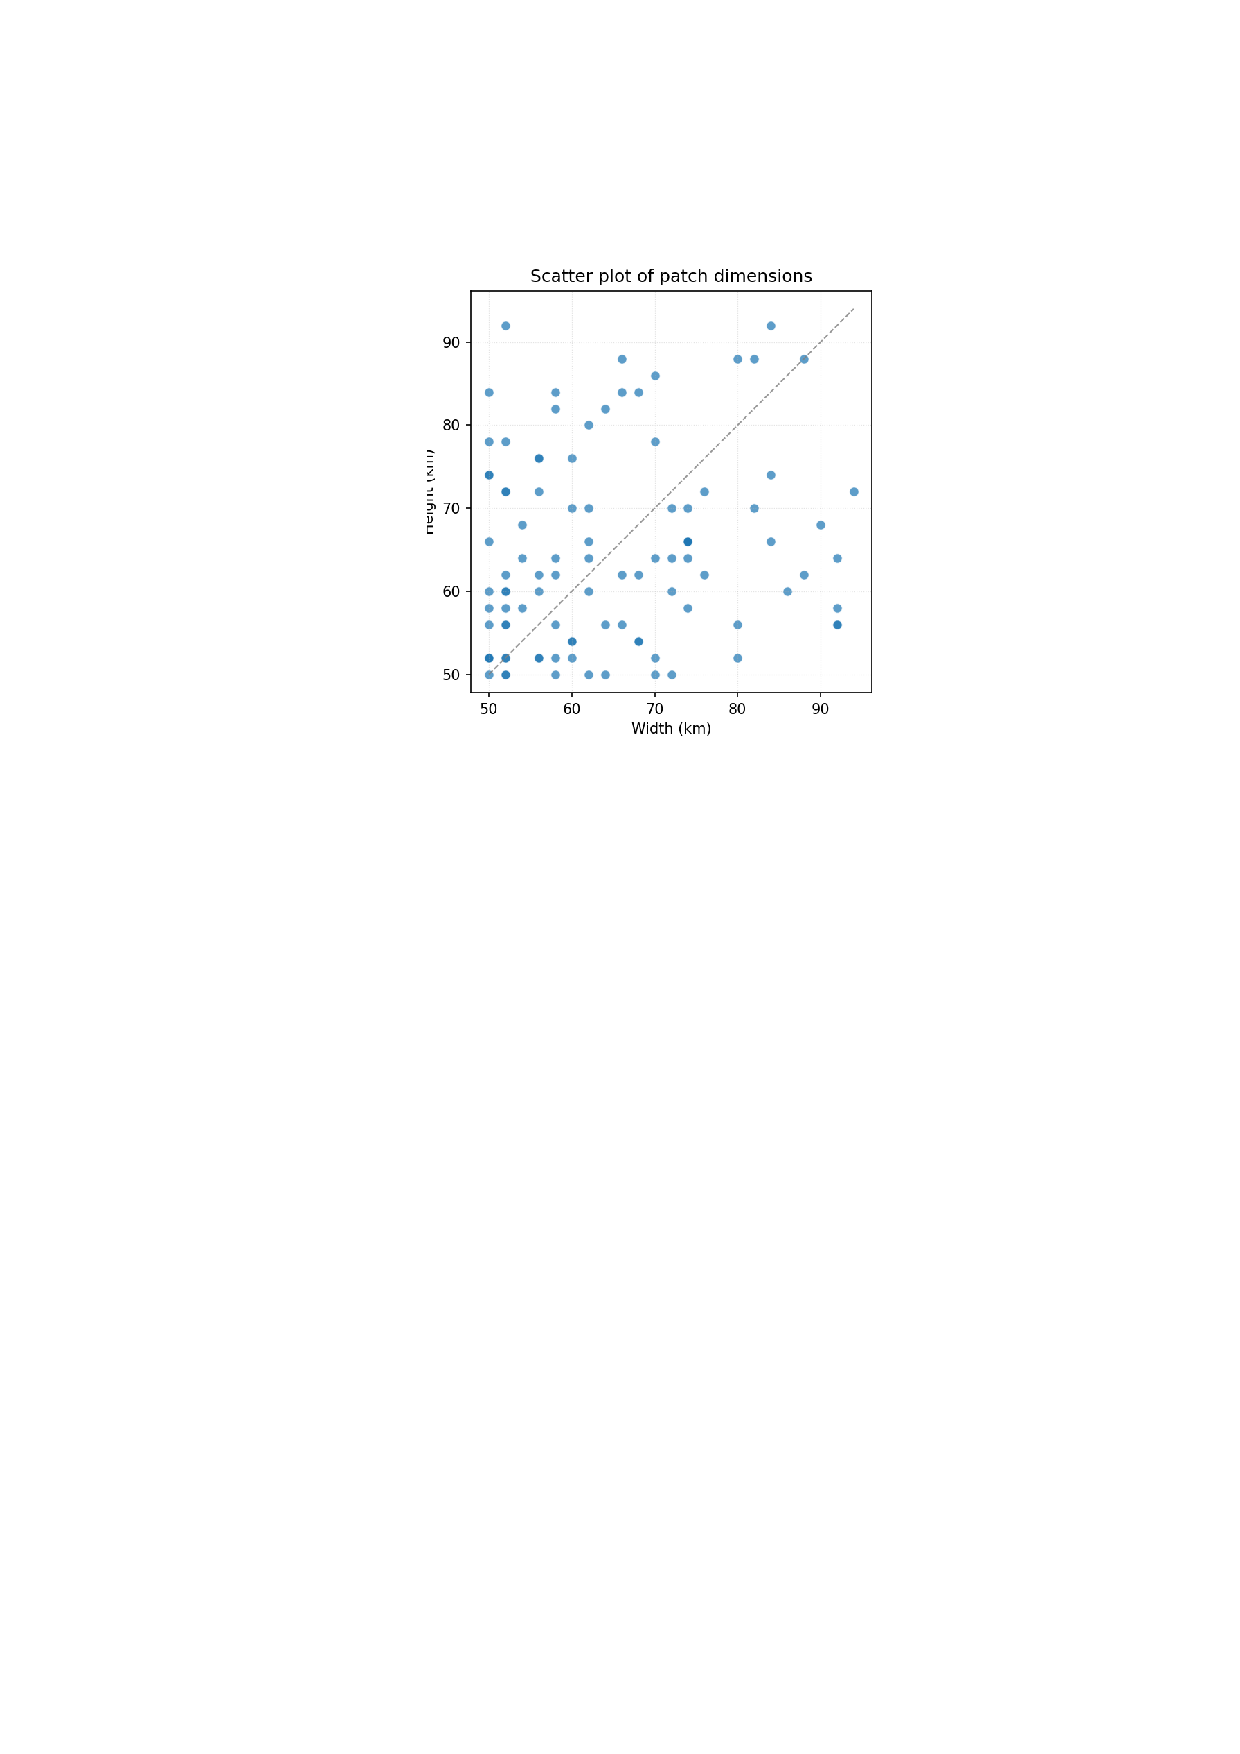
\includegraphics[width=\linewidth]{images/thesis-patch-dimensions.pdf}
\end{column}
\begin{column}{.66\textwidth}
\centering
\vspace{0pt}
\begin{minipage}[c][4.25cm][c]{\linewidth}
\centering
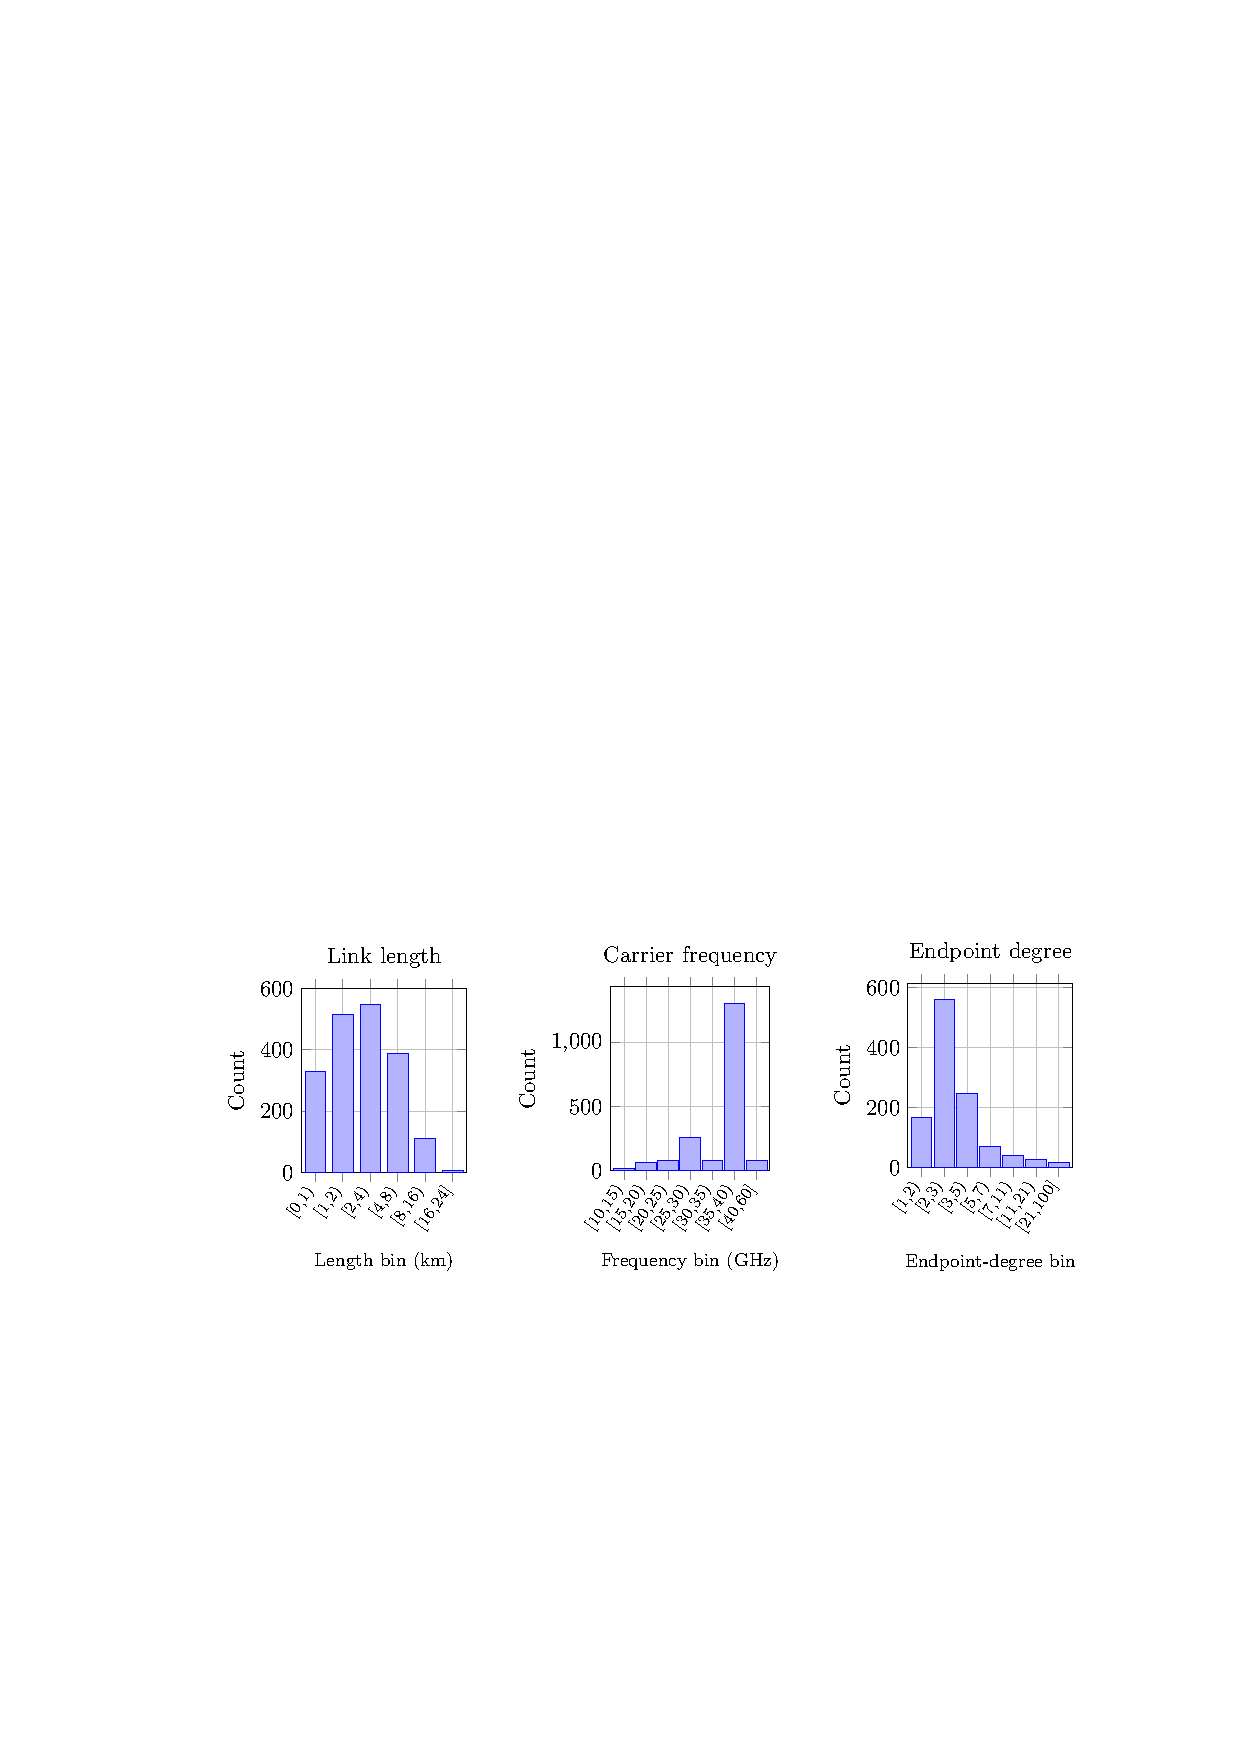
\includegraphics[width=\linewidth]{images/thesis-link-histograms.pdf}
\end{minipage}
\end{column}
\end{columns}
\vspace{-1mm}
{\footnotesize\centering
\textbf{Patch geometry:} all 100 patches
\hfill
\textbf{Link distributions:} largest patch ($88\times88$ km; 1,894 link observations)\par}
\note{The plotted graphics are vector crops taken directly from the thesis PDF: Figure 2 for patch dimensions and Figure A.1 for the three link histograms. They were not redrawn or regenerated. The patch-dimensions plot covers all 100 benchmark patches. The link-network histograms describe the largest patch by physical area: January 29, 2023 at 19:00, 88 km by 88 km. Patch width and height are both 50--95 km; one dot represents one patch and the dashed diagonal marks equal width and height. Length and frequency counts refer to 1,894 link observations, counting two frequencies on the same path as two observations. Endpoint degree is the number of link observations incident to each of the 1,123 distinct endpoint nodes; its histogram therefore sums to 1,123, not 1,894. Key summaries: 73.4\% of link observations are shorter than 4 km, 69.0\% are in the 35--40 GHz band, and 86.7\% of endpoints have degree below five. The link histograms characterize one representative largest patch, not all 100 patches.}
\end{frame}

\begin{comment}
\begin{frame}[t]
\slidetitle{Reference fields and synthetic measurements}
\textbf{Refinement and smoothing}\par
Each 2-km cell becomes $16\times16$ inherited subpixels, at 125-m spacing.
\[R^\star=K_\sigma*R^\uparrow,\qquad
K_\sigma(i,j)=\frac{\exp[-(i^2+j^2)/(2\sigma^2)]}
{\sum_{a,b=-3}^{3}\exp[-(a^2+b^2)/(2\sigma^2)]},\quad\sigma=1.\]
\vspace{2mm}
\textbf{Synthetic attenuation}\par
Overlay the network template and apply the rain-attenuation model to $R^\star$.
\vspace{3mm}
\begin{center}\begin{tabular}{lc}
\toprule Statistic & Value (mm/h)\\\midrule
Mean of the 100 spatial patch means & To be computed\\\bottomrule
\end{tabular}\end{center}
\note{Kernel indices i,j are -3 to 3. Boundary padding uses nearest values. Smoothing is numerical refinement, not a claim of 125-m radar resolution. The intensity statistic includes dry pixels and gives equal weight to each patch. Winter precipitation may include snow. The synthetic experiment treats reference water-equivalent precipitation as liquid rain for attenuation simulation, which does not validate snow attenuation retrieval.}
\end{frame}
\end{comment}

\begin{frame}[t]
\slidetitle{Reconstruction methods}
\vspace{8mm}
\centering
\methodstable{
  \methodrow{IDW}{Use link midpoints as virtual rain gauges; weight observations by distance to the target pixel.}
  \methodrow{ILDW}{Weight observations by distance from the target pixel to the link segment.}
  \methodrow{Optimization}{Estimate pixel rain rates by fitting attenuations while controlling spatial variation.}}
\note{This is the overview of the three reconstruction approaches. The following slides introduce them one at a time, with the active method highlighted. IDW and ILDW interpolate path-average rainfall estimates. Regularized optimization estimates a nonnegative rainfall value in each pixel.}
\end{frame}

\begin{frame}[t]
\slidetitle{Reconstruction methods}
\vspace{8mm}\centering
\methodstable{
  \methodfocusrow{IDW}{Use link midpoints as virtual rain gauges; weight observations by distance to the target pixel.}
  \methodrow{ILDW}{Weight observations by distance from the target pixel to the link segment.}
  \methodrow{Optimization}{Estimate pixel rain rates by fitting attenuations while controlling spatial variation.}}
\end{frame}

\begin{frame}[t]
\slidetitle{IDW: turn each link into a point observation}
\centering\small
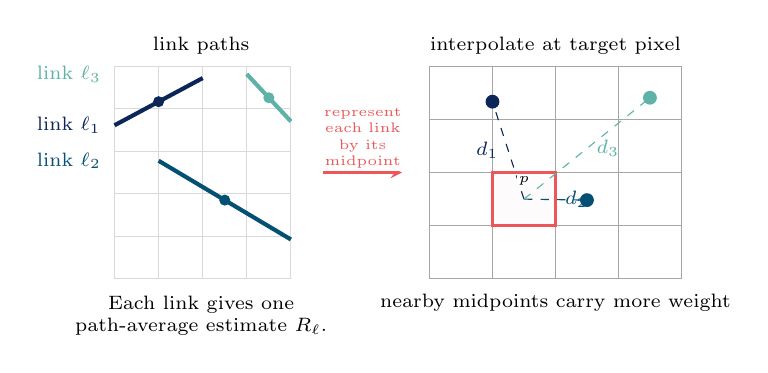
\begin{tikzpicture}[x=1cm,y=1cm,>=stealth,font=\scriptsize]
% Link geometry on a grid, with each virtual midpoint marked on its link
\foreach \x in {0,.56,1.12,1.68,2.24} {\draw[black!15] (\x,.35)--(\x,3.05);}
\foreach \y in {.35,.89,1.43,1.97,2.51,3.05} {\draw[black!15] (0,\y)--(2.24,\y);}
\draw[DarkBlue,line width=1.5pt] (0,2.30)--(1.12,2.90);
\draw[MediumBlue,line width=1.5pt] (.56,1.85)--(2.24,.85);
\draw[MediumGreen,line width=1.5pt] (1.68,2.95)--(2.24,2.35);
\fill[DarkBlue] (.56,2.60) circle (2pt);
\fill[MediumBlue] (1.40,1.35) circle (2pt);
\fill[MediumGreen] (1.96,2.65) circle (2pt);
\node[anchor=east,text=DarkBlue] at (-.05,2.30){link $\ell_1$};
\node[anchor=east,text=MediumBlue] at (-.05,1.85){link $\ell_2$};
\node[anchor=east,text=MediumGreen] at (-.05,2.95){link $\ell_3$};
\node[above] at (1.1,3.08){link paths};
\node[align=center] at (1.1,-.12){Each link gives one\\path-average estimate $R_\ell$.};
\draw[->,thick,MediumRed] (2.65,1.7)--(3.65,1.7)
  node[midway,above,align=center,text width=1.45cm,font=\tiny,fill=white,inner sep=1pt]
  {represent each link\\by its midpoint};
% target grid and virtual stations
\foreach \x in {4.0,4.8,5.6,6.4,7.2} {\draw[black!35] (\x,.35)--(\x,3.05);}
\foreach \y in {.35,1.025,1.70,2.375,3.05} {\draw[black!35] (4.0,\y)--(7.2,\y);}
\fill[DarkBlue] (4.8,2.60) circle (2.5pt);
\fill[MediumBlue] (6.0,1.35) circle (2.5pt);
\fill[MediumGreen] (6.8,2.65) circle (2.5pt);
\fill[MutedRed,opacity=.22] (4.8,1.025) rectangle (5.6,1.70);
\draw[MediumRed,line width=1pt] (4.8,1.025) rectangle (5.6,1.70);
\draw[dashed,DarkBlue] (5.2,1.3625)--(4.8,2.6) node[midway,left]{$d_1$};
\draw[dashed,MediumBlue] (5.2,1.3625)--(6.0,1.35) node[midway,right]{$d_2$};
\draw[dashed,MediumGreen] (5.2,1.3625)--(6.8,2.65) node[midway,right]{$d_3$};
\node[font=\tiny,fill=white,inner sep=.5pt] at (5.2,1.60){$p$};
\node[above] at (5.6,3.08){interpolate at target pixel};
\node[align=center] at (5.6,.05){nearby midpoints carry more weight};
\end{tikzpicture}

\vspace{1mm}
\[
\widehat R(p)=\sum_{\ell\in N_p}w_{p\ell}R_\ell,
\qquad
w_{p\ell}=\frac{d_{p\ell}^{-2}}{\sum_{j\in N_p}d_{pj}^{-2}},
\qquad d_{p\ell}=\|c_p-m_\ell\|_2.
\]
\smallskip
\small $N_p$: link midpoints within 15 km of pixel center $c_p$. Closer midpoint $\Rightarrow$ larger weight.
\note{IDW is applied to the path-average rain-rate estimates derived from each link attenuation. Represent each observation as a virtual point at the link midpoint $m_\ell$. For a target pixel center $c_p$, retain observations within the 15 km cutoff and normalize inverse-square-distance weights. A closer virtual station therefore contributes more. Exact implementation details: if one or more link midpoints fall inside the pixel, the pixel estimate is the mean of those link values instead; if there are no midpoints in the search radius, estimate zero. The illustration omits these edge rules to keep the main idea clear. This is an interpolation baseline, not a joint inversion of all link paths.}
\end{frame}

\begin{frame}[t]
\slidetitle{Discretized IDW: when a pixel contains midpoints}
\begin{columns}[c,onlytextwidth]
\begin{column}{.43\textwidth}
\centering
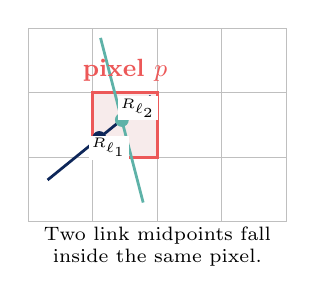
\begin{tikzpicture}[x=0.82cm,y=0.82cm,font=\scriptsize]
\foreach \x in {0,1,2,3,4} {\draw[black!25] (\x,0)--(\x,3);}
\foreach \y in {0,1,2,3} {\draw[black!25] (0,\y)--(4,\y);}
\fill[MutedRed] (1,1) rectangle (2,2);
\draw[MediumRed,line width=1.1pt] (1,1) rectangle (2,2);
\draw[DarkBlue,line width=1pt] (.30,.65)--(1.90,1.95);
\draw[MediumGreen,line width=1pt] (1.12,2.85)--(1.78,.3);
\fill[DarkBlue] (1.10,1.30) circle (2.5pt);
\fill[MediumGreen] (1.45,1.58) circle (2.5pt);
\node[font=\tiny,fill=white,inner sep=1pt] at (1.25,1.15){$R_{\ell_1}$};
\node[font=\tiny,fill=white,inner sep=1pt] at (1.70,1.76){$R_{\ell_2}$};
\node[font=\small\bfseries,text=MediumRed,anchor=south] at (1.5,2.02){pixel $p$};
\node[align=center] at (2,-.38){Two link midpoints fall\\inside the same pixel.};
\end{tikzpicture}
\end{column}
\begin{column}{.57\textwidth}
\textbf{Use the local midpoint observations directly}
\[
\begin{aligned}
M_p&=\{\ell:m_\ell\in p\},\\
\widehat R_p&=\frac{1}{|M_p|}\sum_{\ell\in M_p}R_\ell,
\qquad M_p\ne\varnothing.
\end{aligned}
\]
\vspace{1mm}
Here $R_\ell$ is link $\ell$'s rain-rate estimate. If several midpoints fall in pixel $p$, average those estimates.

\vspace{3mm}
\begin{beamercolorbox}[rounded=true,sep=1.2ex,wd=\linewidth]{block body example}
\small
An occupied pixel gets a direct local estimate. Use distance-weighted IDW only when no midpoint falls inside.
\end{beamercolorbox}
\end{column}
\end{columns}
\note{This is the discretized midpoint rule implemented by our IDW baseline. First convert each link attenuation to a path-equivalent rain-rate value R_ell and place it at the link midpoint m_ell. For pixel p, form M_p from all links whose midpoints lie inside that pixel. If M_p is nonempty, assign p the arithmetic mean of those values, regardless of the midpoint-to-pixel-center distances. This handles the case where a midpoint lands inside a grid cell (including avoiding a zero-distance singularity if a midpoint coincides with the pixel center) and gives local observations direct influence on their containing cell. That intuition is a rationale for the rule, while the code and thesis specify the rule itself rather than documenting the original design motivation. For empty pixels, use the truncated inverse-square IDW rule from the previous slide using midpoints within 15 km; if none lie in range, return zero.}
\end{frame}

\begin{frame}[t]
\slidetitle{Reconstruction methods}
\vspace{8mm}\centering
\methodstable{
  \methodrow{IDW}{Use link midpoints as virtual rain gauges; weight observations by distance to the target pixel.}
  \methodfocusrow{ILDW}{Weight observations by distance from the target pixel to the link segment.}
  \methodrow{Optimization}{Estimate pixel rain rates by fitting attenuations while controlling spatial variation.}}
\end{frame}

\begin{frame}[t]
\slidetitle{(Discretized) ILDW: distance to each link}
\begin{columns}[T,onlytextwidth]
\begin{column}{.53\textwidth}
\centering
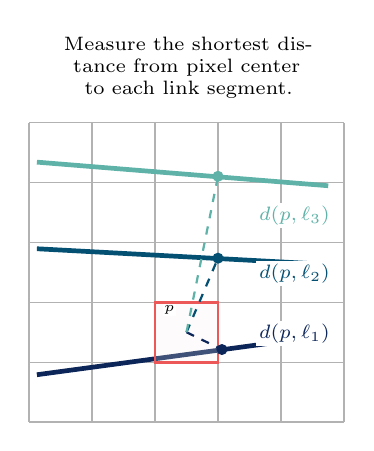
\begin{tikzpicture}[x=1cm,y=1cm,>=stealth,font=\scriptsize]
\foreach \x in {0,.8,1.6,2.4,3.2,4.0} {\draw[black!30] (\x,0)--(\x,3.8);}
\foreach \y in {0,.76,1.52,2.28,3.04,3.8} {\draw[black!30] (0,\y)--(4.0,\y);}
\draw[DarkBlue,line width=1.7pt] (.1,.6)--(3.8,1.1);
\draw[MediumBlue,line width=1.7pt] (.1,2.2)--(3.8,2.0);
\draw[MediumGreen,line width=1.7pt] (.1,3.3)--(3.8,3.0);
\fill[MutedRed,opacity=.22] (1.6,.76) rectangle (2.4,1.52);
\draw[MediumRed,line width=1pt] (1.6,.76) rectangle (2.4,1.52);
\fill[DarkBlue] (2.45,.92) circle (2pt);
\fill[MediumBlue] (2.4,2.08) circle (2pt);
\fill[MediumGreen] (2.4,3.12) circle (2pt);
\draw[dashed,DarkBlue,thick] (2.0,1.14)--(2.45,.92);
\draw[dashed,MediumBlue,thick] (2.0,1.14)--(2.4,2.08);
\draw[dashed,MediumGreen,thick] (2.0,1.14)--(2.4,3.12);
\node[DarkBlue,anchor=west,fill=white,inner sep=1pt] at (2.88,1.12){$d(p,\ell_1)$};
\node[MediumBlue,anchor=west,fill=white,inner sep=1pt] at (2.88,1.88){$d(p,\ell_2)$};
\node[MediumGreen,anchor=west,fill=white,inner sep=1pt] at (2.88,2.62){$d(p,\ell_3)$};
\node[font=\tiny,fill=white,inner sep=.5pt] at (1.78,1.42){$p$};
\node[align=center,text width=3.8cm] at (2,4.5){Measure the shortest distance from pixel center to each link segment.};
\end{tikzpicture}
\end{column}
\begin{column}{.45\textwidth}
\small
Same link-level rain estimates and inverse-square rule as IDW; only the distance changes:
\[
d_{p\ell}=\operatorname{dist}(c_p,\ell),\qquad
w_{p\ell}=\frac{d_{p\ell}^{-2}}{\sum_{j\in N_p}d_{pj}^{-2}}.
\]
\[
\widehat R(p)=\sum_{\ell\in N_p}w_{p\ell}R_\ell.
\]
\footnotesize If a link crosses the pixel, average the crossing links; otherwise use links within 15 km.
\end{column}
\end{columns}
\note{ILDW uses exactly the same link rain-rate observations, inverse-square exponent, 15 km cutoff, and normalized weighted average as IDW. Its geometric difference is to calculate point-to-segment distance from the pixel center to the actual line segment, instead of distance to the midpoint. A special crossing-pixel rule avoids a zero-distance singularity: if one or more links cross the pixel, average those links' estimates. This is our link-aware interpolation variant.}
\end{frame}

\begin{frame}[t]
\slidetitle{Reconstruction methods}
\vspace{8mm}\centering
\methodstable{
  \methodrow{IDW}{Treat each link midpoint as a virtual rain gauge.}
  \methodrow{ILDW}{Weight observations by distance to the link segment.}
  \methodfocusrow{Optimization}{Estimate pixel rain rates by fitting attenuations while controlling spatial variation.}}
\end{frame}

\begin{frame}[t]
\slidetitle{Optimization}
\centering
\vspace{1mm}
Using L-BFGS-B, we estimate a nonnegative rain rate in every pixel by minimizing
\[
J(r)=\alpha_{\rm atten}J_{\rm atten}(r)
+\alpha_{1d}J_{1d}(r)+\alpha_{2d}J_{2d}(r)
+\textcolor{MediumRed}{\alpha_{\rm total}J_{\rm total}(r)},
\qquad r\geq0.
\]
\vspace{-1mm}
\small
\renewcommand{\arraystretch}{1.15}
\begin{tabular}{p{0.21\textwidth}p{0.70\textwidth}}
$J_{\rm atten}$ & Fits predicted link attenuations to the observations.\\
$J_{1d}$ & Penalizes differences between neighbouring pixels.\\
$J_{2d}$ & Penalizes changes in those differences, discouraging curvature and oscillation.\\
$J_{\rm total}$ & Penalizes mean squared rain rate, weakly shrinking the field toward zero.\\
\end{tabular}
\vspace{1mm}
\small\par For each patch, the weights use the cost values at the ILDW estimate:
\[
\begin{aligned}
\alpha_{\rm atten}&=\frac{1}{J_{\rm atten}(r_{\rm ILDW})},&
\alpha_{1d}&=\frac{1}{J_{1d}(r_{\rm ILDW})},\\[-1mm]
\alpha_{2d}&=\frac{1}{2J_{2d}(r_{\rm ILDW})},&
\alpha_{\rm total}&=\frac{1}{|P|J_{\rm total}(r_{\rm ILDW})}.
\end{aligned}
\]
\vspace{-1mm}
\scriptsize\textcolor{MediumRed}{In our experiments, the $J_{\rm total}$ term did not noticeably affect reconstruction quality.}
\note{For each patch P, the optimization variables are the nonnegative pixel values r. The attenuation term measures link mismatch, normalized by path length and averaged over links. J_1d is the mean squared first difference over horizontal and vertical neighbors. J_2d is the mean squared second difference over collinear pixel triples. J_total is mean squared rain rate. The weights are heuristic, instance-wise normalization choices based on term values at the ILDW solution: alpha_atten=1/J_atten(ILDW), alpha_1d=1/J_1d(ILDW), alpha_2d=1/(2 J_2d(ILDW)), and alpha_total=(1/|P|)/J_total(ILDW). Thus alpha_2d halves the second-difference contribution relative to the first-difference term, while the extra 1/|P| makes the total-rain shrinkage weak. The red emphasis signals that J_total is included but intentionally weak: it gently discourages overly large rain rates and is not meant to dominate attenuation matching or spatial regularization. These weights make magnitudes comparable at the reference solution; they were not selected by a systematic sensitivity sweep. The full cost definitions and exact normalizations are in the thesis.}
\end{frame}

% Detailed numerical counterexample retained, but hidden for now.
\begin{comment}
\begin{frame}[t]
\slidetitle{A counterexample to convexity}
\small
One horizontal link crosses the middle row of a $3\times3$ grid.
\[R^{(L)}=\begin{bmatrix}1&1&1\\20&1&1\\1&1&1\end{bmatrix},\qquad
R^{(R)}=\begin{bmatrix}1&1&1\\1&1&20\\1&1&1\end{bmatrix},\qquad
R^{(M)}=\frac{R^{(L)}+R^{(R)}}2.\]
Both endpoint fields produce $A_{\rm obs}=0.80155$ dB.
\[J_{\rm atten}(R)=\frac{(\widehat A(R)-A_{\rm obs})^2}{|\ell|},\qquad
J_{\rm atten}(R^{(L)})=J_{\rm atten}(R^{(R)})=0.\]
For $0<\alpha<1$, strict concavity gives $2(10.5)^\alpha>20^\alpha+1$.
\[J_{\rm atten}(R^{(M)})=0.0050431>\frac{J_{\rm atten}(R^{(L)})+J_{\rm atten}(R^{(R)})}{2}=0.\]
\note{Exact example supplied by the user: 38.003 GHz, horizontal polarization, kappa=0.400171594750, alpha=0.881535333268, d_p=0.125 km for each crossed pixel, link length=0.375 km. Midpoint attenuation=0.845082934781 dB. This proves nonconvexity of the attenuation term for this instance. It does not automatically prove nonconvexity of every possible fully regularized objective.}
\end{frame}
\end{comment}

\begin{frame}[t]
\slidetitle{Problem: nonconvex attenuation fit}
\centering
The attenuation-mismatch objective is
\[J_{\rm atten}(r)=\sum_{\ell}\bigl(\widehat A_\ell(r)-A_\ell\bigr)^2.\]
With the power-law forward model, this objective \textbf{can be nonconvex} when a link's exponent $\alpha_\ell\ne1$.
\vspace{2mm}
\begin{columns}[T]
\begin{column}{0.47\textwidth}
\textbf{Why it matters}
\begin{itemize}
\item Optimization may settle at a local solution.
\item The result may depend on the starting rain field.
\end{itemize}
\end{column}
\begin{column}{0.48\textwidth}
\centering
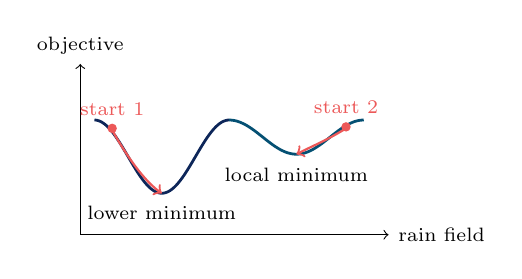
\begin{tikzpicture}[x=0.9cm,y=0.62cm,font=\scriptsize]
\draw[->] (-2,0)--(2.35,0) node[right]{rain field};
\draw[->] (-2,0)--(-2,3.5) node[above,align=center]{objective};
\draw[DarkBlue,line width=1pt,smooth,domain=90:450,samples=90]
  plot({-1.8+(\x-90)/360*1.9},{2.35+0.75*(sin(\x)-1)});
\draw[MediumBlue,line width=1pt,smooth,domain=90:450,samples=90]
  plot({0.1+(\x-90)/360*1.9},{2.35+0.35*(sin(\x)-1)});
\fill[MediumRed] (-1.55,2.18) circle (1.7pt);
\fill[MediumRed] (1.75,2.21) circle (1.7pt);
\draw[->,MediumRed,thick] (-1.55,2.14)..controls(-1.28,1.45)and(-1.05,1.05)..(-0.85,0.85);
\draw[->,MediumRed,thick] (1.75,2.18)..controls(1.50,1.95)and(1.25,1.8)..(1.05,1.65);
\node[MediumRed,anchor=south] at (-1.55,2.25){start 1};
\node[MediumRed,anchor=south] at (1.75,2.28){start 2};
\node[anchor=north] at (-0.85,0.78){lower minimum};
\node[anchor=north] at (1.05,1.57){local minimum};
\end{tikzpicture}
\end{column}
\end{columns}
\note{The qualitative schematic was redrawn by the author from collaborator-provided material. The attenuation-mismatch term can be nonconvex for the nonlinear power-law model; nonlinear alone is not a proof, and the separate commented-out 3x3 example gives a concrete counterexample. The schematic illustrates a possible optimization landscape, not measured solver trajectories. Initialization can affect which local solution an iterative method finds.}
\end{frame}

\begin{frame}[t]
\slidetitle{Convex surrogate using virtual links}
\small
\textbf{1. Choose a nearly linear reference model.} At $f_0=24.92$ GHz with horizontal polarization, ITU-R gives $\alpha_0\approx1$. In the surrogate, set $\alpha_0=1$:
\[\widehat A_\ell^0(r)=\kappa_0\int_\ell r(s)\,\mathrm ds
=\kappa_0\sum_p d_{\ell,p}r_p.\]

\textbf{2. Convert each observation to an equivalent uniform rain rate.}
\[r_\ell^{\rm eq}=\left(\frac{A_\ell^{\rm obs}/|\ell|}{\kappa_\ell}\right)^{1/\alpha_\ell},
\qquad A_\ell^0=\kappa_0r_\ell^{\rm eq}|\ell|.\]
The virtual link keeps the original path geometry and uses the same equivalent rain rate.

\textbf{3. Fit the virtual-link attenuations.}
\[J_0(r)=\sum_\ell\bigl(\widehat A_\ell^0(r)-A_\ell^0\bigr)^2.\]
Since $\widehat A_\ell^0(r)$ is linear in $r$, this least-squares term is convex. Adding convex smoothness and shrinkage terms preserves convexity; a positive $\ell_2$ shrinkage term makes the surrogate strictly convex.
\note{The explanation draws on collaborator-provided material. $A_\ell^{\rm obs}$ is the observed total rain-induced attenuation at the original link frequency and polarization; dividing by path length and applying the inverse ITU power law yields the uniform rain-equivalent rate. The virtual observation $A_\ell^0$ is computed at the reference frequency using that same equivalent rate and original geometry. The surrogate sets $\alpha_0=1$ exactly, motivated by the near-unity ITU exponent at 24.92 GHz for horizontal polarization; this is an approximation. The attenuation least-squares term is convex because its forward map is linear. Convex regularizers preserve convexity; the positive squared-$\ell_2$ shrinkage makes the full surrogate strictly convex. This does not imply the original-frequency objective is convex or that homotopy finds its global optimum.}
\end{frame}

\begin{frame}[t]
\slidetitle{Homotopy continuation}
\centering
Rather than switch directly to the nonlinear original model, gradually interpolate each link's frequency:
\[
f_\ell^\lambda=(1-\lambda)f^0+\lambda f_\ell,
\qquad \lambda=0,0.1,\ldots,1.
\]
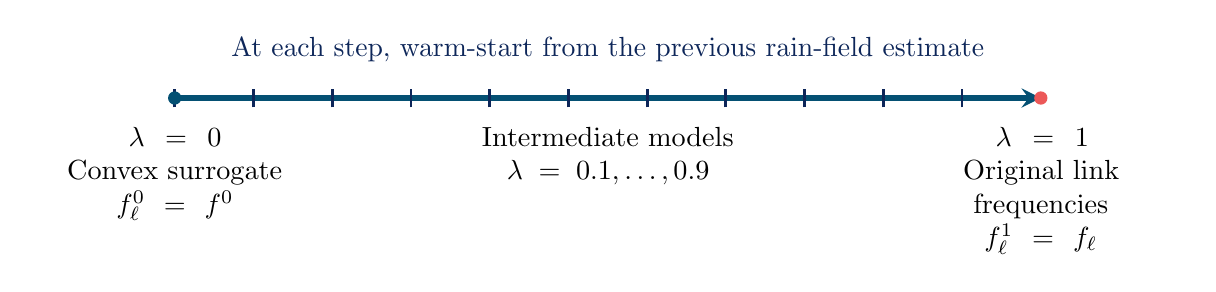
\begin{tikzpicture}[x=1cm,y=1cm,>=stealth]
  \draw[->,line width=2pt,draw=MediumBlue] (0,0)--(11,0);
  \foreach \x in {0,1,...,10} {
    \draw[DarkBlue,line width=1pt] (\x,-0.12)--(\x,0.12);
  }
  \fill[MediumBlue] (0,0) circle (2.4pt);
  \fill[MediumRed] (11,0) circle (2.4pt);
  \node[align=center,anchor=north,text width=3.5cm] at (0,-0.25)
    {$\lambda=0$\\Convex surrogate\\$f_\ell^0=f^0$};
  \node[align=center,anchor=north,text width=4.0cm] at (5.5,-0.25)
    {Intermediate models\\$\lambda=0.1,\ldots,0.9$};
  \node[align=center,anchor=north,text width=3.5cm] at (11,-0.25)
    {$\lambda=1$\\Original link frequencies\\$f_\ell^1=f_\ell$};
  \node[align=center,text=DarkBlue] at (5.5,0.62)
    {At each step, warm-start from the previous rain-field estimate};
\end{tikzpicture}
\vspace{1mm}
\textcolor{black!70}{Continuation reaches the original model, but does not guarantee its global optimum.}
\note{Homotopy Solver begins with the convex virtual-link problem at $\lambda=0$ and advances through ten stages using $\delta=0.1$. At each stage, interpolate frequency while retaining each link's geometry, length, and polarization. Recompute the ITU-R coefficients and virtual attenuation observations from the link's uniform rain-equivalent rate. Solve the current regularized objective with L-BFGS-B, initializing the first stage from the constant 0.6 mm/h field and every later stage from the previous stage's solution. The attenuation-weight normalization is recomputed for the current stage using the ILDW rainfall field as its reference. At $\lambda=1$, frequencies equal the original link frequencies and the final estimate is $\widehat r^1$. This continuation strategy may help the optimizer track a solution path, but it does not guarantee a global optimum of the original nonconvex objective. Thesis source: Latex/main.tex, Homotopy Solver subsection.}
\end{frame}

\begin{frame}[t]
\frametitle{Evaluation metrics}
Let $R_i$ and $\hat R_i$ be the reference and reconstructed rain rates at pixel $i$, for $n$ paired pixels.
\[\mathrm{Bias}=\frac1n\sum_{i=1}^n(\hat R_i-R_i)\qquad\text{\footnotesize mean signed error}\]
\[\mathrm{RMSE}=\sqrt{\frac1n\sum_{i=1}^n(\hat R_i-R_i)^2}\qquad\text{\footnotesize root mean squared error}\]
Both metrics have units of mm/h. Positive bias means overestimation.

\vspace{2mm}
\textbf{Pearson correlation.} Do above- and below-average rainfall occur in the same locations in both maps?
\[\rho=\frac{\sum_i(\hat R_i-\bar{\hat R})(R_i-\bar R)}{\sqrt{\sum_i(\hat R_i-\bar{\hat R})^2}\sqrt{\sum_i(R_i-\bar R)^2}}.\]
\note{Pearson correlation describes whether the spatial patterns vary together. Near +1 means above-average and below-average areas tend to line up; near 0 means little linear pattern association; near -1 means they tend to reverse. Correlation does not measure absolute agreement or overall bias.}
\end{frame}

\begin{frame}[t]
\slidetitle{Whole-patch reconstruction results}
\centering\small
\renewcommand{\arraystretch}{1.35}
\begin{tabular}{lccc}
\toprule Method & RMSE (mm/h) & Signed bias (mm/h) & Pearson $r$\\\midrule
IDW & $1.307\pm1.234$ & $0.034\pm0.296$ & $0.866\pm0.059$\\
ILDW & $1.239\pm1.182$ & $0.047\pm0.261$ & $0.878\pm0.055$\\
Solver(ILDW) & $1.059\pm1.192$ & $0.040\pm0.235$ & $0.918\pm0.055$\\
Convex Solver & $0.845\pm0.803$ & $0.023\pm0.075$ & $0.940\pm0.034$\\
Homotopy Solver & $0.845\pm0.803$ & $0.023\pm0.075$ & $0.940\pm0.034$\\
Solver(GT) & $0.503\pm0.369$ & $0.009\pm0.030$ & $0.961\pm0.032$\\\bottomrule
\end{tabular}
\par\vspace{5mm}\normalsize
Mean $\pm$ standard deviation across 100 patches.
\par\vspace{3mm}
Solver(GT) is an optimistic diagnostic, initialized from the reference field.
\note{Exact values from Latex/main.tex, table tab:patch_map_metrics. Use these thesis values rather than differently rounded values shown in an earlier collaborator presentation. Signed bias is distinct from mean absolute patch bias. Similar Convex and Homotopy summaries do not imply identical fields.}
\end{frame}

\begin{frame}[t]
\slidetitle{Paired comparison: Convex Solver vs IDW}
\centering
\vspace{4mm}
\small
\renewcommand{\arraystretch}{1.5}
\begin{tabular}{@{}l c c c p{.37\textwidth}@{}}
\toprule
Metric & Better direction & Convex wins & IDW wins & Patch-level evidence\\
\midrule
RMSE & lower & 100 & 0 & All patches favor Convex Solver\\
Absolute bias & lower & 78 & 22 & Reject null: $p=4.667\times10^{-7}$\\
Pearson correlation & higher & 100 & 0 & All patches favor Convex Solver\\
\bottomrule
\end{tabular}
\par\vspace{4mm}
\footnotesize Paired, one-sided $t$-test on 100 patches for absolute-bias difference $d_P=|{\rm Bias}_{P,\rm Convex}|-|{\rm Bias}_{P,\rm IDW}|$, with $H_0:\mathbb{E}[d_P]\geq0$.
\note{Paired, one-sided Student t-tests on patch-level differences from the PatchMapMetrics_ByPatch sheet in Compute-Link-Attenuations/HundredPatches/pipeline/report/stats.xlsx. For RMSE test d=RMSE_IDW-RMSE_Convex >0: t(99)=9.2953, p=1.8848e-15; wins 100/100. For correlation test d=r_Convex-r_IDW >0: t(99)=22.0828, p=2.4572e-40; wins 100/100. For absolute bias test d=|Bias_IDW|-|Bias_Convex| >0: t(99)=5.2335, p=4.6668e-7; wins 78/100. These are one-sided tests in the expected improvement direction, unadjusted for testing three metrics. The p-values assume independent patchwise paired differences; possible spatial/temporal dependence in the benchmark means they should be interpreted cautiously. Absolute bias is not the same as signed bias.}
\end{frame}

\begin{frame}[t]
\slidetitle{Taylor diagram: aggregate across 100 patches}
\begin{columns}[T,onlytextwidth]
\begin{column}{.53\textwidth}
\centering
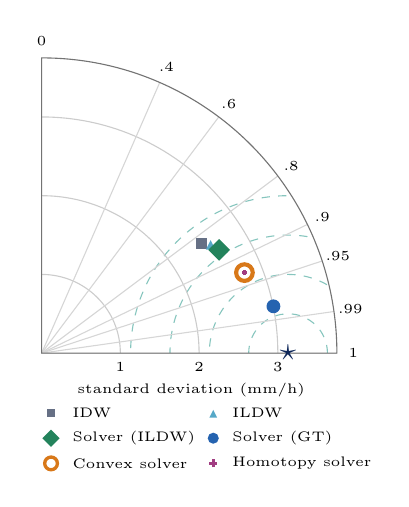
\begin{tikzpicture}[x=1cm,y=1cm,font=\scriptsize]
% Unnormalized Taylor geometry: radius is SD (mm/h), angle is correlation.
\begin{scope}
\clip (0,0) rectangle (3.75,3.75);
\clip (0,0) circle (3.75);
\foreach \e in {.5,1,1.5,2} {
  \draw[MediumGreen,dashed,opacity=.75] (3.130,0) circle (\e);
}
\end{scope}
\foreach \r in {1,2,3} {\draw[black!20] (\r,0) arc (0:90:\r);}
\foreach \corr/\ang in {0/90,.4/66.42,.6/53.13,.8/36.87,.9/25.84,.95/18.19,.99/8.11,1/0} {
  \draw[black!16] (0,0)--(\ang:3.75);
  \node[font=\tiny] at ({3.96*cos(\ang)},{3.96*sin(\ang)}) {\corr};
}
\draw[black!55] (0,0)--(3.75,0) arc (0:90:3.75)--cycle;
\foreach \r in {1,2,3} {\node[below,font=\tiny] at (\r,0) {\r};}
\node[font=\tiny,anchor=north] at (1.9,-.25){standard deviation (mm/h)};
% Aggregate method points: (x,y)=(F rho, F sqrt(1-rho^2)).
\node[rectangle,fill=TaylorIDW,inner sep=2pt] at (2.034,1.393) {};
\fill[TaylorILDW] (2.146,1.436)--(2.086,1.316)--(2.206,1.316)--cycle;
\node[diamond,fill=TaylorSolverILDW,inner sep=2pt] at (2.255,1.312) {};
\fill[TaylorSolverGT] (2.944,.595) circle (2.5pt);
\draw[TaylorConvex,line width=1.5pt] (2.576,1.023) circle (3pt);
\draw[TaylorHomotopy,line width=1.2pt] (2.546,1.022)--(2.606,1.022);
\draw[TaylorHomotopy,line width=1.2pt] (2.576,.992)--(2.576,1.052);
\node[text=DarkBlue] at (3.130,0){\large$\star$};
% Compact legend, two columns.
\node[rectangle,fill=TaylorIDW,inner sep=1.6pt] at (.12,-.76) {};
\node[anchor=west,font=\tiny] at (.27,-.76){IDW};
\fill[TaylorILDW] (2.18,-.72)--(2.13,-.82)--(2.23,-.82)--cycle;
\node[anchor=west,font=\tiny] at (2.30,-.76){ILDW};
\node[diamond,fill=TaylorSolverILDW,inner sep=1.6pt] at (.12,-1.08) {};
\node[anchor=west,font=\tiny] at (.27,-1.08){Solver (ILDW)};
\fill[TaylorSolverGT] (2.18,-1.08) circle (2pt);
\node[anchor=west,font=\tiny] at (2.30,-1.08){Solver (GT)};
\draw[TaylorConvex,line width=1.2pt] (.12,-1.40) circle (2.3pt);
\node[anchor=west,font=\tiny] at (.27,-1.40){Convex solver};
\draw[TaylorHomotopy,line width=1pt] (2.13,-1.40)--(2.23,-1.40);
\draw[TaylorHomotopy,line width=1pt] (2.18,-1.45)--(2.18,-1.35);
\node[anchor=west,font=\tiny] at (2.30,-1.40){Homotopy solver};
\end{tikzpicture}
\vspace{.5mm}
\scriptsize
$\theta=\arccos\rho$: correlation; $F$: SD (mm/h). Star: reference
$(0,G)$. Dashed arcs: centered RMSE (mm/h).
\end{column}
\begin{column}{.45\textwidth}
\small
\footnotesize
\begin{itemize}
  \setlength{\itemsep}{2pt}
  \item Each point summarizes 100 equally weighted patches.
  \item For patch $k$, $g_k$ is the ground-truth rain map and $f_k$ its reconstruction.
  \item Center each map by its own mean; compute $G_k=\operatorname{SD}(g_k)$, $F_k=\operatorname{SD}(f_k)$, and $\rho_k=\operatorname{corr}(g_k,f_k)$.
\end{itemize}
{\footnotesize
\[
\begin{aligned}
G&=\sqrt{\tfrac1{100}\textstyle\sum_k G_k^2},\\
F&=\sqrt{\tfrac1{100}\textstyle\sum_k F_k^2},\\
C&=\tfrac1{100}\textstyle\sum_k G_kF_k\rho_k,\\
\rho&=\frac{C}{GF},\\
(\theta,r)&=(\arccos\rho,\,F).
\end{aligned}
\]
}
\end{column}
\end{columns}
\note{The normalized aggregate diagram is removed; this is the physical-units summary. For each of 100 patches, subtract the reference map's own mean and the reconstruction's own mean, then calculate population standard deviations G_k and F_k and covariance C_k. Give every patch equal weight: G and F are root-mean-square standard deviations, while C is mean covariance. The plotted aggregate correlation is C/(GF), with radius F and angle arccos(rho). The reference star is at radius G and angle zero. The dashed centered-RMSE contours are at E=sqrt(F^2+G^2-2C), equivalently the RMS of the patch-level centered RMSE values. Thus the aggregate point is not the arithmetic mean of the 100 individual Taylor points. The quantities G,F,E have units mm/h; mean bias is excluded and is reported in the metric table.}
\end{frame}

\begin{frame}[t]
\slidetitle{Taylor diagrams by reconstruction method}
\centering
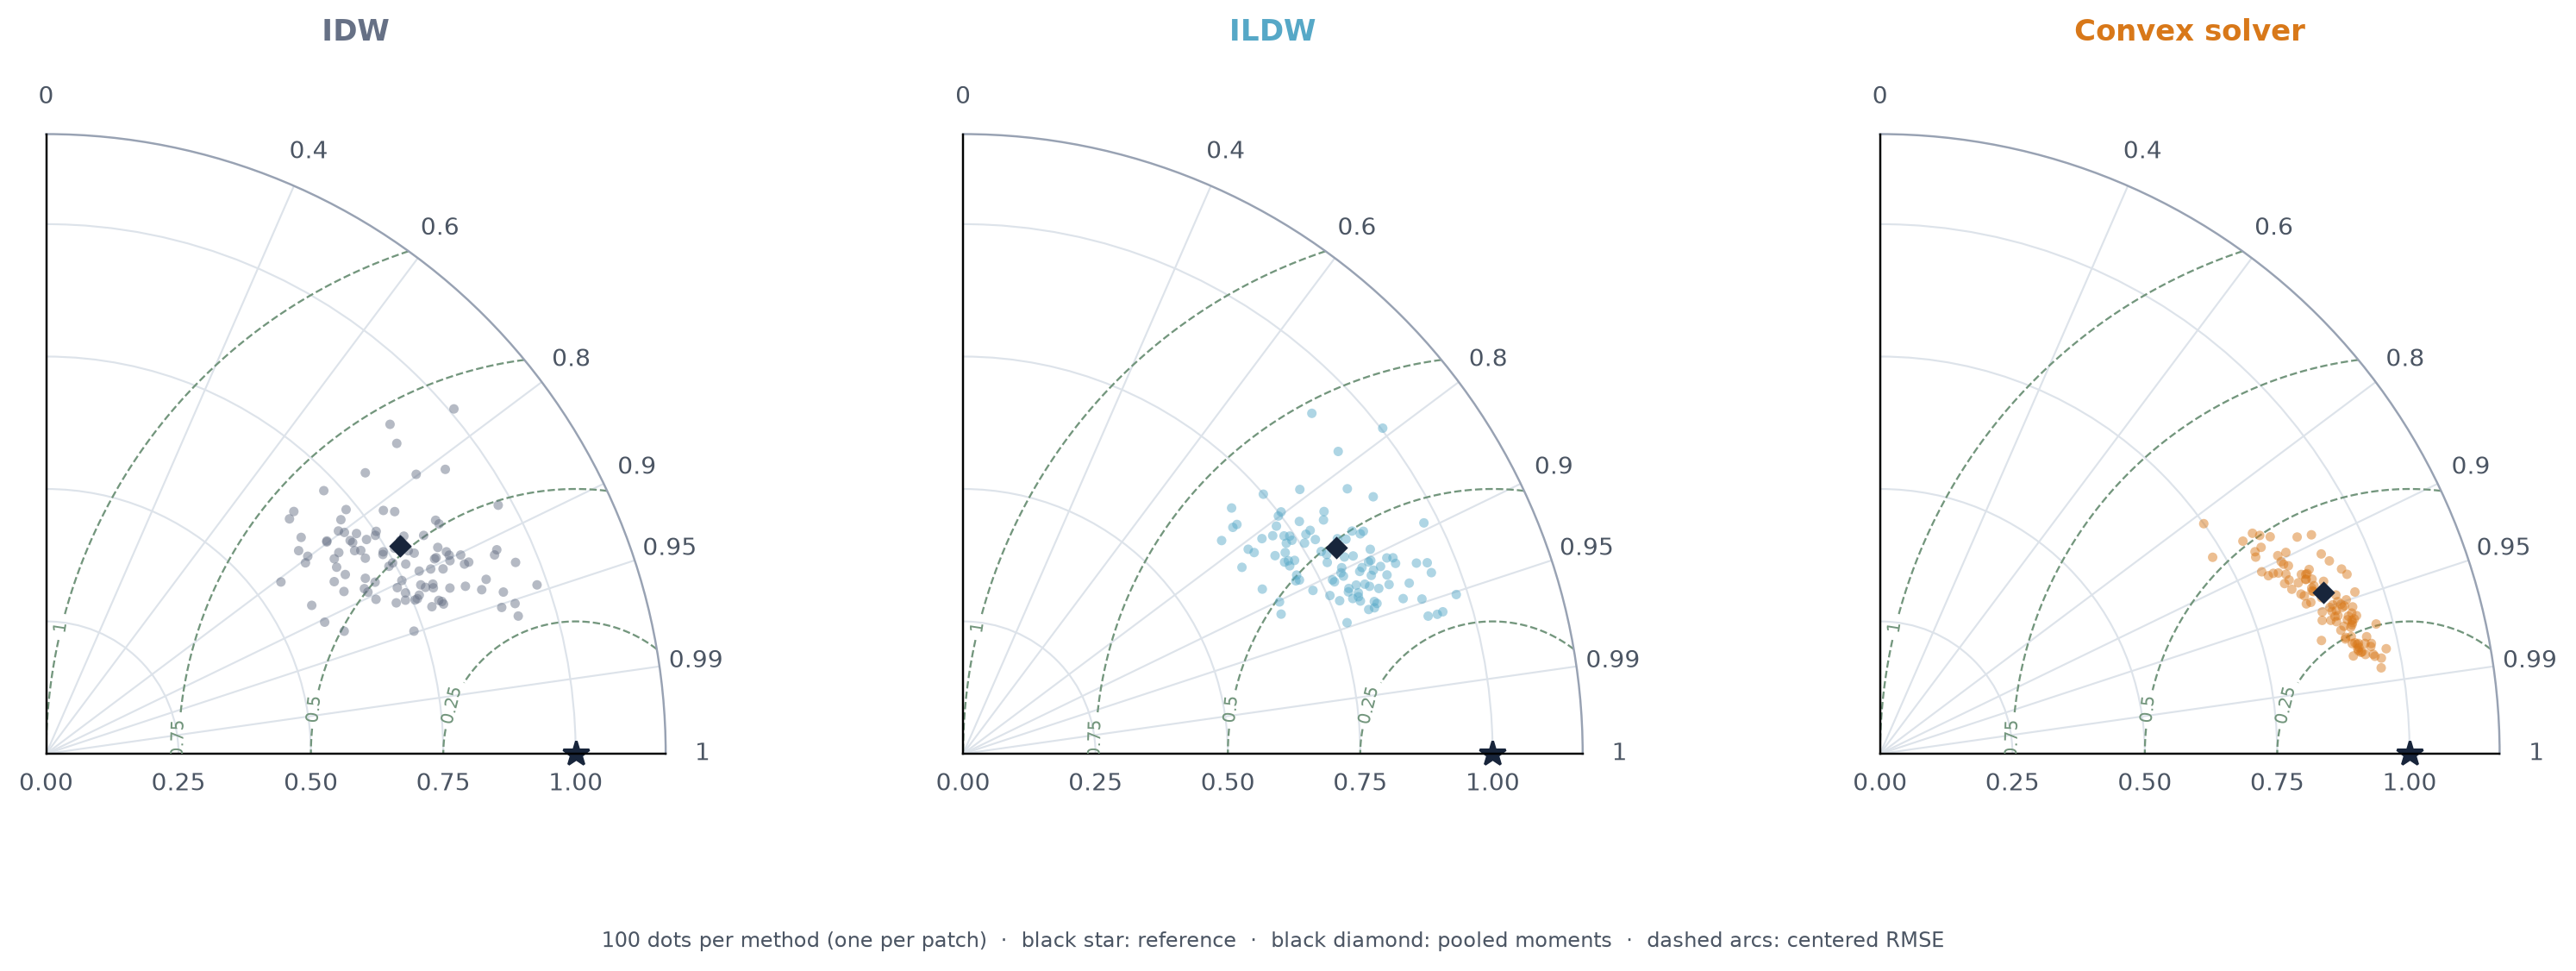
\includegraphics[width=\textwidth,height=.70\textheight,keepaspectratio]{taylor-selected-patch-clouds.png}
\vspace{-1mm}
\small
Each dot is one patch; the black diamond summarizes the 100 patches.\par
\note{These are patch-level normalized Taylor diagrams for IDW, ILDW, and Convex Solver, all using the same 100 patches. A dot is one patch, the black star is the reference point (correlation 1 and normalized standard deviation 1), and the black diamond is the aggregate pooled moment. The angle encodes correlation; radius is the model/reference standard-deviation ratio; dashed contours indicate centered RMSE. Bias is removed by centering and cannot be read from these plots. Solver(GT) and Homotopy Solver are omitted here for brevity and may be included if desired later.}
\end{frame}

\begin{frame}[t]
\slidetitle{Reconstruction error over rainy pixels}
\begin{columns}[T,onlytextwidth]
\begin{column}{.64\textwidth}
\centering
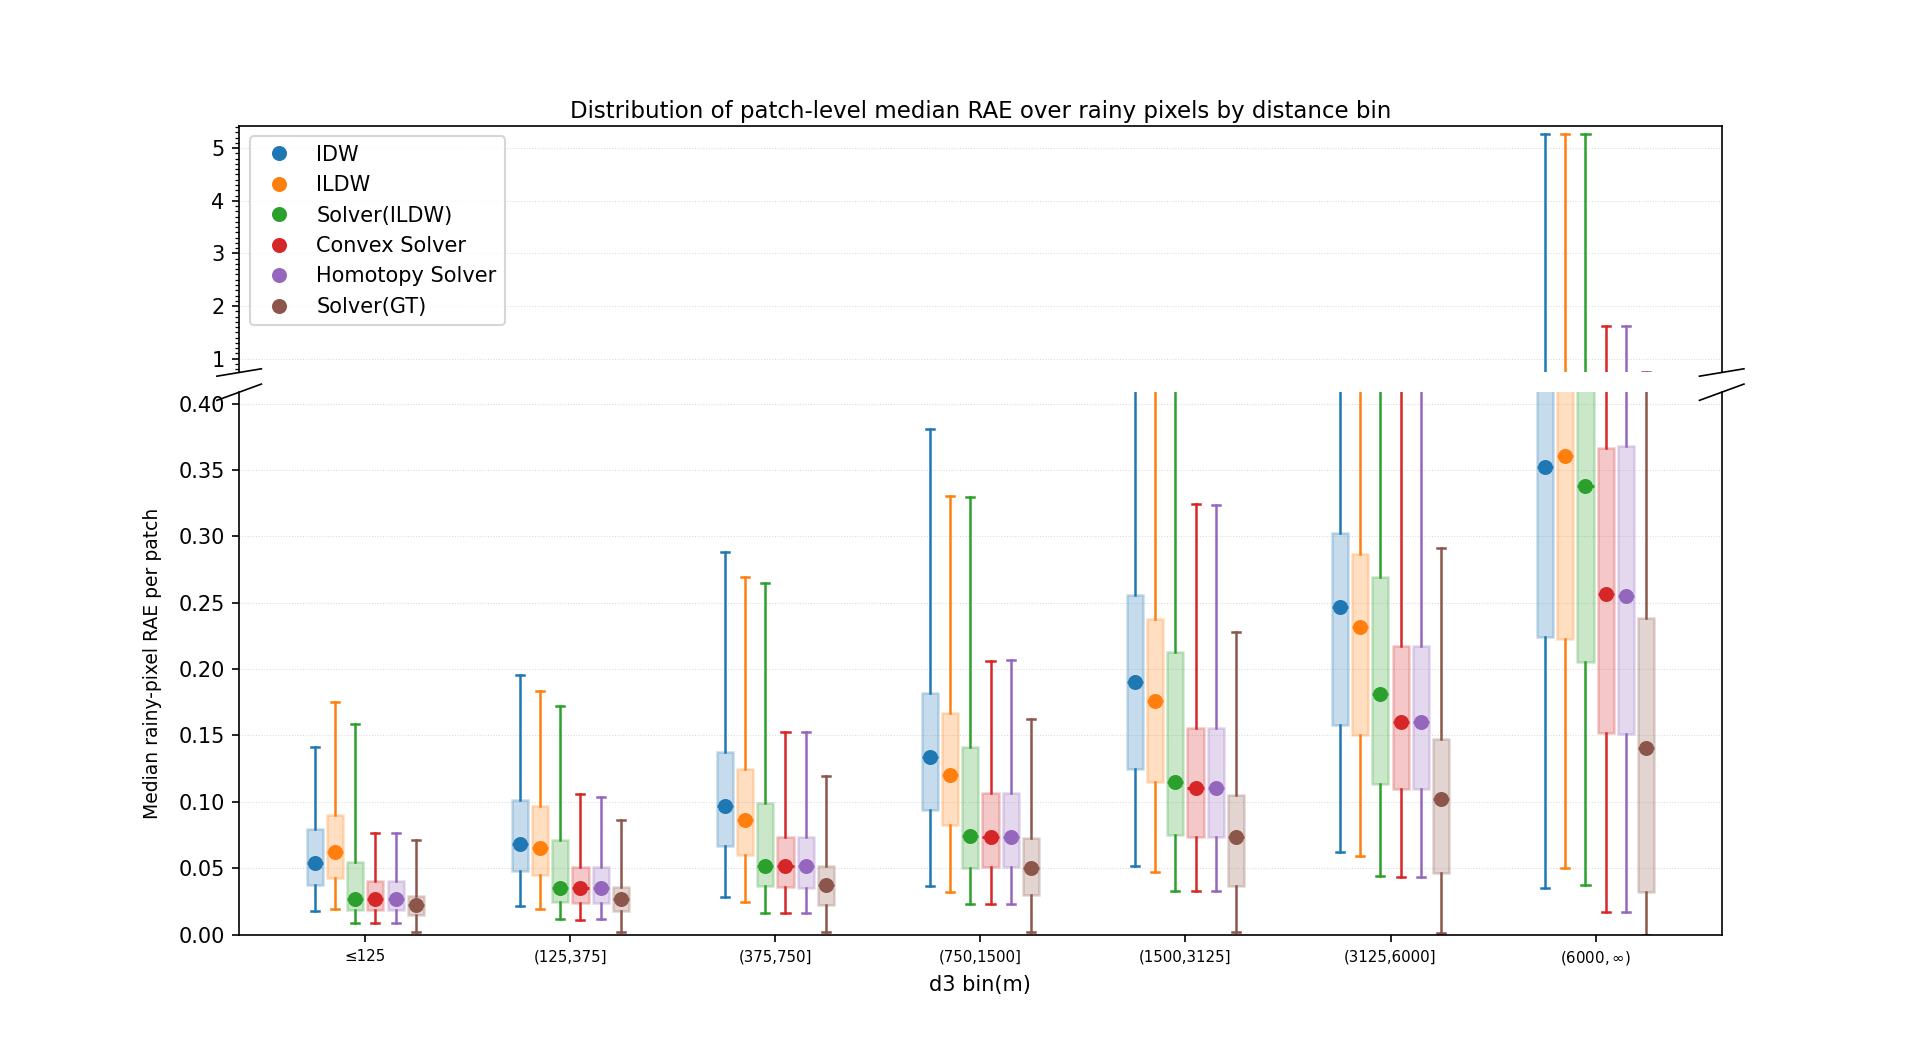
\includegraphics[width=\linewidth]{distance-rainy.png}
\end{column}
\begin{column}{.36\textwidth}
\centering\scriptsize
Mean wet pixels per patch\\
Total: 238,922\\[1mm]
\setlength{\tabcolsep}{2pt}
\begin{tabular}{lrr}
\toprule
$d_3$ bin (m) & Pixels & \% total\\\midrule
$\leq125$ & 4,267 & 1.8\\
125--375 & 16,738 & 7.0\\
375--750 & 26,810 & 11.2\\
750--1500 & 51,989 & 21.8\\
1500--3125 & 88,839 & 37.2\\
3125--6000 & 45,929 & 19.2\\
$>6000$ & 4,350 & 1.8\\
\bottomrule
\end{tabular}
\end{column}
\end{columns}
\vspace{1mm}\centering\footnotesize Wet pixels ($R\geq0.6$ mm/h); relative absolute error by distance to the third-closest link.\\
\note{The two panels in the source figure show the full error range (top) and a detail view (bottom), to make the near-zero distributions legible despite large-distance outliers. Rainy pixels are classified from the reference field at the 0.6 mm/h threshold. Per pixel relative absolute error is $|R-\widehat R|/R$; within each patch and distance bin, the median is computed, then the figure summarizes those patch medians. $d_3$ is distance from a pixel center to its third-closest link segment. The patch-level view is useful because it reveals how reconstruction error changes with link coverage, instead of only reporting one all-pixel score. This distance-conditioned analysis is a contribution of this evaluation; avoid claiming no prior work has done it without a systematic literature comparison.}
\end{frame}

\begin{frame}[t]
\slidetitle{Reconstruction error over dry pixels}
\begin{columns}[T,onlytextwidth]
\begin{column}{.64\textwidth}
\centering
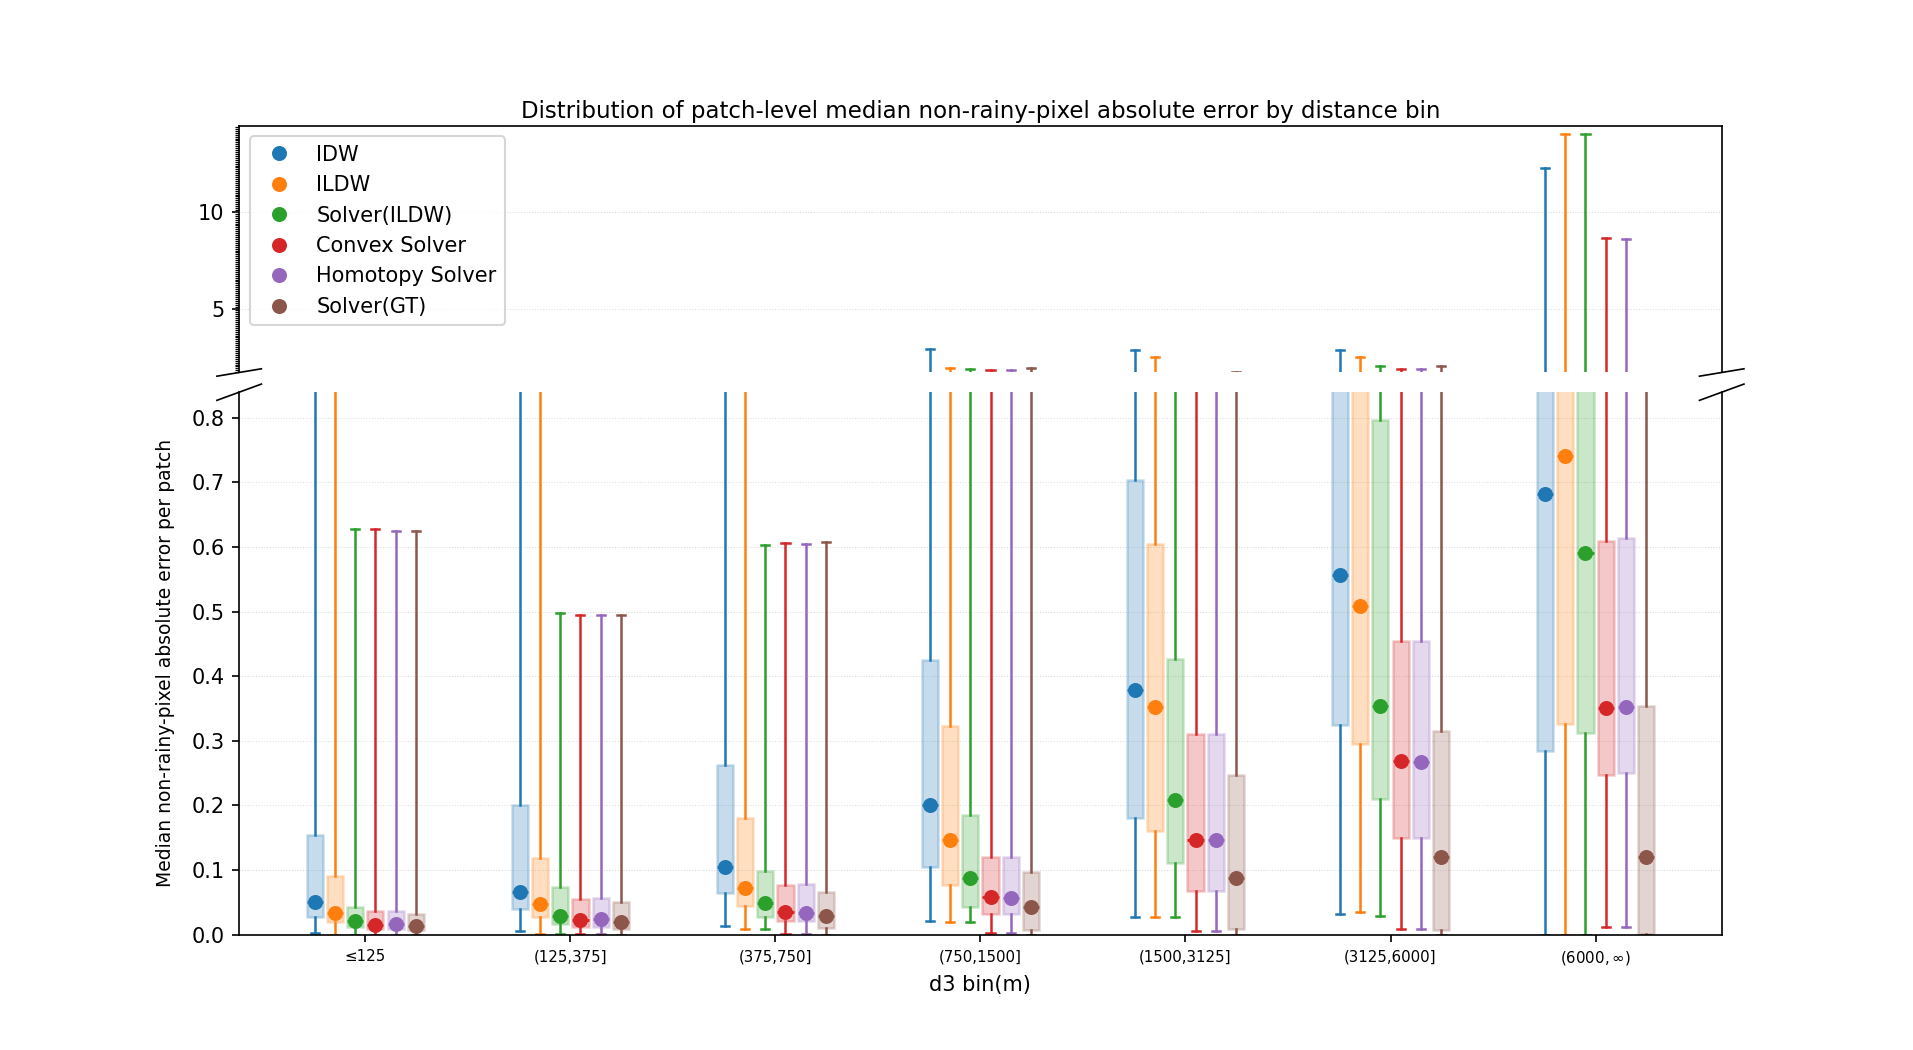
\includegraphics[width=\linewidth]{distance-dry.png}
\end{column}
\begin{column}{.36\textwidth}
\centering\scriptsize
Mean dry pixels per patch\\
Total: 30,569\\[1mm]
\setlength{\tabcolsep}{2pt}
\begin{tabular}{lrr}
\toprule
$d_3$ bin (m) & Pixels & \% total\\\midrule
$\leq125$ & 564 & 1.8\\
125--375 & 2,261 & 7.4\\
375--750 & 3,389 & 11.1\\
750--1500 & 6,447 & 21.1\\
1500--3125 & 10,776 & 35.3\\
3125--6000 & 6,197 & 20.3\\
$>6000$ & 936 & 3.1\\
\bottomrule
\end{tabular}
\end{column}
\end{columns}
\vspace{1mm}\centering\footnotesize Dry pixels ($R<0.6$ mm/h); absolute error by distance to the third-closest link.\\
\note{The two panels in the source figure show full range (top) and detail view (bottom). Dry/non-rainy pixels are reference pixels with $R<0.6$ mm/h. Relative error is unstable or undefined near zero, so absolute error $|R-\widehat R|$ in mm/h is used. As in the rainy plot, first compute the median per patch and distance bin, then summarize those patch medians across patches. The rightmost bins have fewer contributing patches (as shown under each bin), so their summaries are less stable. The wet/dry threshold is an analysis convention, not a universal meteorological boundary.}
\end{frame}

\begin{frame}[t]
\slidetitle{Wet/dry classification at 0.6 mm/h}
\centering\small
\renewcommand{\arraystretch}{1.3}
\begin{tabular}{lrr}
\toprule
Method & False-positive rate & False-negative rate\\
 & (of reference-dry pixels) & (of reference-wet pixels)\\
\midrule
IDW & 59.8\% & 0.3\%\\
ILDW & 56.2\% & 0.4\%\\
Solver (ILDW init.) & 46.3\% & 0.4\%\\
Convex solver & 40.0\% & 0.5\%\\
Homotopy solver & 40.1\% & 0.5\%\\
Solver (GT init.) & 33.1\% & 0.3\%\\
\bottomrule
\end{tabular}
\par\vspace{4mm}
\normalsize
On average, only \textbf{10.5\%} of reference pixels are dry\par
($R<0.6$ mm/h); the benchmark is strongly rain-dominated.
\par\vspace{2mm}
\footnotesize FPR = predicted wet among reference-dry pixels; FNR = predicted dry among reference-wet pixels.
\note{Entries are mean patchwise conditional rates from the saved wet/dry confusion summary at threshold 0.6 mm/h. FPR=FP/(FP+TN), conditional on reference-dry pixels; FNR=FN/(FN+TP), conditional on reference-wet pixels. These are not the false-wet/false-dry fractions of all pixels. The mean reference-dry share is 10.5\% across patches (patchwise pixel proportions averaged equally), so the reference-wet share is about 89.5\%. The Solver(GT init.) is an optimistic diagnostic initialized using ground truth, not a deployable method. Polz et al. (2020) is relevant but not an exact derivation of this threshold: their study labels link-time windows wet at path-average rain rate >=0.1 mm/h, and separately reports that over 90\% of periods above 0.6 mm/h were detected. Thus 0.6 mm/h is a defensible practical threshold for evaluating reliably detectable rainfall, but it should be presented as our chosen evaluation cutoff, not as Polz's formal wet/dry definition or a universal standard. Citation: Polz et al., Atmospheric Measurement Techniques 13, 3835--3853 (2020), doi:10.5194/amt-13-3835-2020.}
\end{frame}

\begin{frame}[t]
\slidetitle{End-to-end reconstruction runtime}
\centering\small
\renewcommand{\arraystretch}{1.35}
\begin{tabular}{lcccc}
\toprule
Solver & Mean $\pm$ SD (s) & Median (s) & Range (s) & Optimizer time$^{*}$ (s)\\
\midrule
IDW & $7.53\pm2.43$ & $7.10$ & $4.01$--$14.18$ & ---\\
ILDW & $18.69\pm6.20$ & $18.25$ & $8.67$--$38.19$ & ---\\
Convex solver & $76.03\pm27.08$ & $71.31$ & $32.76$--$153.12$ & $57.00\pm22.35$\\
\bottomrule
\end{tabular}
\par\vspace{3mm}
\normalsize All times are per patch (100 patches); optimizer time is reported for the Convex Solver.
\par\vspace{2mm}
\footnotesize Optimizer time covers the solver call; end-to-end time also includes loading, setup, diagnostics, and saving.\\
Sequential runs on an Apple M2 MacBook Air (8-core CPU, 8 GB RAM).
\note{Values reproduced from the thesis runtime table (Latex/main.tex, tab:runtime_summary) and convex_solver_runtime_summary.json. This was a focused timing experiment for IDW, ILDW, and Convex Solver only; Solver(ILDW), Homotopy Solver, and Solver(GT) were not timed in that experiment. End-to-end wall-clock time per patch includes loading, initialization, reconstruction, diagnostics, and writing output. For the Convex Solver, optimizer time is the time spent inside the scipy.optimize.minimize call running L-BFGS-B: mean 56.9979 s, sample SD 22.3511 s, median 51.1527 s, range 17.6129--118.6051 s across 100 patches. L-BFGS-B is a limited-memory quasi-Newton algorithm: it iteratively improves the solution using a compact approximation of curvature information and supports bound constraints; here, the bounds keep pixel rain rates nonnegative. The 100 patches/methods were processed sequentially on an Apple M2 MacBook Air, 8-core CPU, 8 GB memory. These are machine- and implementation-specific reference timings, not a controlled comparison at equal accuracy or a claim about operational latency.}
\end{frame}



\begin{frame}[t]
\slidetitle{Conclusions and outlook}
\begin{beamercolorbox}[rounded=true,sep=1.5ex,wd=\textwidth]{block body example}
\centering\large
On our \textbf{synthetic benchmark}, Convex Solver improves map-level scores over IDW.\par
\smallskip\normalsize\small Does that advantage persist with real network measurements? We have not tested that yet.
\end{beamercolorbox}
\vspace{3mm}
\begin{columns}[T,onlytextwidth]
\begin{column}{.32\textwidth}
\begin{block}{1. Validate in practice}
Use measured CML signal levels and compare with IDW.
\end{block}
\end{column}
\begin{column}{.32\textwidth}
\begin{block}{2. Test other seasons}
Compare maps across seasons: the winter benchmark is largely stratiform, while summer may include more convective rain.
\end{block}
\end{column}
\begin{column}{.32\textwidth}
\begin{block}{3. Learn rainfall structure}
Our current model uses explicit regularization, not a data-learned rainfall prior. Use rainfall maps to learn spatial patterns, while still requiring estimates to match the measured link attenuation.
\end{block}
\end{column}
\end{columns}
\note{The present benchmark simulates attenuations from EURADCLIM fields and realistic link geometry; it does not test operational signal-level measurements. Thus the observed advantage over IDW is a synthetic-benchmark result, not evidence yet of superiority in deployment. Practical validation should handle measured dry baselines, wet antenna attenuation, noise, and quality-control effects. Temporal extension idea: reconstruct $\widehat R_t$ at successive times; estimate a motion field $v_t$ (for example, with optical flow) from consecutive reconstructions; advect the field to form a nowcast; when measurements at a future time arrive, use them to update the forecast/reconstruction and repeat. This is a proposed direction, not an implemented experiment. The current objective uses explicit smoothness/shrinkage regularizers and does not learn a prior distribution from rainfall examples. Future work could learn a spatial prior from data and combine it with the physical attenuation likelihood, e.g. in a Bayesian formulation. Avoid claiming that most/all existing methods learn such priors; this slide only contrasts our current formulation with that possible extension.}
\end{frame}

\begin{frame}[t]
\slidetitle{A plausible CML-only use case: data-sparse African cities}
\small
\textbf{Ouagadougou, Burkina Faso:} the clearest documented example.
\vspace{1mm}
\begin{table}
\centering
\renewcommand{\arraystretch}{1.25}
\begin{tabular}{p{0.29\textwidth}p{0.66\textwidth}}
\toprule
\textbf{Evidence} & \textbf{Reported detail}\\
\midrule
CML rainfall map & 100 unique paths; 5-min, 0.55-km grid (2020)\\
Gauge use & One reference gauge for evaluation, not a map input\\
Signal-data access & $>1{,}000$ links nationwide at 1-min sampling (2020--21); about 300 around Ouagadougou\\
Other cities & Niamey: 190 links; Douala: 227 links\\
Observation gap & Radar data not operationally available in Sahel; gauge networks sparse\\
Counts not reported & Comparable citywide gauge totals and radar footprints\\
\bottomrule
\end{tabular}
\end{table}
\vspace{-1mm}
\begin{beamercolorbox}[rounded=true,sep=1ex,wd=\textwidth]{block body example}
\centering
\textbf{Use case:} reconstruct local rain fields from link attenuation when radar is unavailable and gauges are too sparse to resolve storm patterns.
\end{beamercolorbox}
\vspace{1mm}
\scriptsize Link counts come from different studies and network footprints. ``CML-only'' means links are the only local input to the reconstruction; satellite products may still exist.
\note{Evidence: Djibo et al. (2023), “High-Resolution Rainfall Maps from Commercial Microwave Links for a Data-Scarce Region in West Africa,” Journal of Hydrometeorology, DOI 10.1175/JHM-D-23-0015.1. Their 2020 Ouagadougou maps used rainfall information on 100 unique link paths at 5-min and 0.55-km resolution. One rain gauge was available for reference/validation; it was not an input to the CML map. Turko et al. (2021), “Rainfall Measurement from Commercial Microwave Links for Urban Hydrology in Africa: A Simulation Framework for Sensitivity Analysis,” Journal of Hydrometeorology, DOI 10.1175/JHM-D-20-0163.1. Reports a simulated Ouagadougou urban network geometry of 75 links over a 1250 km^2 domain, and actual available urban networks of 190 links in Niamey and 227 in Douala; densities are described as typical of African cities. Mou et al. (2023), “Towards Innovative Solutions for Monitoring Precipitation in Poorly Instrumented Regions: Real-Time System for Collecting Power Levels of Microwave Links of Mobile Phone Operators for Rainfall Quantification in Burkina Faso,” Systems, DOI 10.3390/systems11010004. Reports an acquisition system collecting one-minute data from over 1000 national links in 2020--2021, including about 300 around Ouagadougou. Sahel radar unavailability and sparse gauge networks are discussed by Doumounia et al. (2014), DOI 10.1002/2014GL060724, and Moumouni et al. (2020), PIAHS 383, 237--244. The cited city studies do not give comparable, exhaustive citywide gauge totals or current radar footprint coverage for Ouagadougou, Niamey, and Douala. Hence the slide presents them as plausible CML-only reconstruction settings, not proof of zero gauges/radars or sole operational rainfall data.}
\end{frame}

% End references and credits. Individual figure credits remain on their slides.
\newcommand{\refentry}[2]{\par\noindent\hangindent=1.1em\hangafter=1 #1\,#2\par\vspace{1.4mm}}
\newcommand{\doiref}[1]{{\tiny\color{black!55}doi:\href{https://doi.org/#1}{#1}}}

\begin{frame}[t]
\slidetitle{References | Early attenuation research}
\begin{columns}[T,onlytextwidth]
\begin{column}{.49\textwidth}
\footnotesize
\refentry{Ryde, J. W. (1946).}{“The attenuation of centimetre radio waves and the echo intensities resulting from atmospheric phenomena.” \emph{J. Inst. Electr. Eng.}, 93(1), 101--103. \doiref{10.1049/JI-3A-1.1946.0029}}
\refentry{Gunn, K. L. S., \& East, T. W. R. (1954).}{“The microwave properties of precipitation particles.” \emph{Q. J. R. Meteorol. Soc.}, 80(346), 522--545. \doiref{10.1002/qj.49708034603}}
\refentry{Atlas, D., \& Ulbrich, C. W. (1977).}{“Path- and area-integrated rainfall measurement by microwave attenuation in the 1--3 cm band.” \emph{J. Appl. Meteorol.}, 16(12), 1322--1331. \doiref{10.1175/1520-0450(1977)016<1322:PAAIRM>2.0.CO;2}}
\end{column}
\begin{column}{.49\textwidth}
\footnotesize
\refentry{Olsen, R. L., Rogers, D. V., \& Hodge, D. B. (1978).}{“The $aR^b$ relation in the calculation of rain attenuation.” \emph{IEEE Trans. Antennas Propag.}, 26(2), 318--329. \doiref{10.1109/TAP.1978.1141845}}
\refentry{Giuli, D. et al. (1991).}{“Tomographic reconstruction of rainfall fields through microwave attenuation measurements.” \emph{J. Appl. Meteorol.}, 30(9), 1323--1340. \doiref{10.1175/1520-0450(1991)030<1323:TRORFT>2.0.CO;2}}
\refentry{Holt, A. R. et al. (2000).}{“Measurement of rainfall by dual-wavelength microwave attenuation.” \emph{Electron. Lett.}, 36(25), 2099--2101. \doiref{10.1049/el:20001468}}
\end{column}
\end{columns}
\end{frame}

\begin{frame}[t]
\slidetitle{References | Commercial-link rainfall mapping}
\begin{columns}[T,onlytextwidth]
\begin{column}{.49\textwidth}
\footnotesize
\refentry{Rahimi, A. R. et al. (2003).}{“The use of dual-frequency microwave links for measuring path-averaged rainfall.” \emph{J. Geophys. Res. Atmos.}, 108(D15), 4467. \doiref{10.1029/2002JD003202}}
\refentry{Upton, G. J. G. et al. (2005).}{“Microwave links: the future for urban rainfall measurement?” \emph{Atmos. Res.}, 77(1--4), 300--312. \doiref{10.1016/j.atmosres.2004.10.009}}
\refentry{Messer, H., Zinevich, A., \& Alpert, P. (2006).}{“Environmental monitoring by wireless communication networks.” \emph{Science}, 312(5774), 713. \doiref{10.1126/science.1120034}}
\refentry{Leijnse, H., Uijlenhoet, R., \& Stricker, J. N. M. (2007).}{“Rainfall measurement using radio links from cellular communication networks.” \emph{Water Resour. Res.}, 43(3), W03201. \doiref{10.1029/2006WR005631}}
\end{column}
\begin{column}{.49\textwidth}
\footnotesize
\refentry{Overeem, A., Leijnse, H., \& Uijlenhoet, R. (2013).}{“Country-wide rainfall maps from cellular communication networks.” \emph{PNAS}, 110(8), 2741--2745. \doiref{10.1073/pnas.1217961110}}
\refentry{Overeem, A., Leijnse, H., \& Uijlenhoet, R. (2016).}{“Two and a half years of country-wide rainfall maps using radio links from commercial cellular networks.” \emph{Water Resour. Res.}, 52(10), 8039--8065. \doiref{10.1002/2016WR019412}}
\refentry{Graf, M. et al. (2020).}{“Rainfall estimation from a German-wide commercial microwave link network.” \emph{Hydrol. Earth Syst. Sci.}, 24, 2931--2950. \doiref{10.5194/hess-24-2931-2020}}
\refentry{Chwala, C., \& Kunstmann, H. (2019).}{“Commercial microwave link networks for rainfall observation: assessment of the current status and future challenges.” \emph{WIREs Water}, 6(2), e1337. \doiref{10.1002/wat2.1337}}
\end{column}
\end{columns}
\end{frame}

\begin{frame}[t]
\slidetitle{References | Reconstruction methods}
\begin{columns}[T,onlytextwidth]
\begin{column}{.49\textwidth}
\footnotesize
\refentry{International Telecommunication Union (2005).}{Recommendation ITU-R P.838-3, “Specific attenuation model for rain for use in prediction methods.” \href{https://www.itu.int/rec/R-REC-P.838-3-200503-I/en}{ITU recommendation}.}
\refentry{Shepard, D. (1968).}{“A two-dimensional interpolation function for irregularly-spaced data.” In \emph{Proc. 23rd ACM National Conf.}, 517--524. \doiref{10.1145/800186.810616}}
\refentry{Eshel, A. et al. (2020).}{“Spatial reconstruction of rain fields from wireless telecommunication networks: scenario-dependent analysis of IDW-based algorithms.” \emph{IEEE Geosci. Remote Sens. Lett.}, 17(5), 770--774. \doiref{10.1109/LGRS.2019.2935348}}
\end{column}
\begin{column}{.49\textwidth}
\footnotesize
\refentry{Eshel, A. et al. (2021).}{“Quantitative analysis of the performance of spatial interpolation methods for rainfall estimation using commercial microwave links.” \emph{J. Hydrometeorol.}, 22(4), 831--843. \doiref{10.1175/JHM-D-20-0164.1}}
\refentry{Byrd, R. H. et al. (1995).}{“A limited memory algorithm for bound constrained optimization.” \emph{SIAM J. Sci. Comput.}, 16(5), 1190--1208. \doiref{10.1137/0916069}}
\refentry{Zhu, C. et al. (1997).}{“Algorithm 778: L-BFGS-B.” \emph{ACM Trans. Math. Softw.}, 23(4), 550--560. \doiref{10.1145/279232.279236}}
\refentry{Allgower, E. L., \& Georg, K. (2003).}{\emph{Introduction to Numerical Continuation Methods}. SIAM. \doiref{10.1137/1.9780898719154}}
\end{column}
\end{columns}
\end{frame}

\begin{frame}[t]
\slidetitle{References | Evaluation and outlook}
\begin{columns}[T,onlytextwidth]
\begin{column}{.49\textwidth}
\footnotesize
\refentry{Taylor, K. E. (2001).}{“Summarizing multiple aspects of model performance in a single diagram.” \emph{J. Geophys. Res. Atmos.}, 106(D7), 7183--7192. \doiref{10.1029/2000JD900719}}
\refentry{Polz, J. et al. (2020).}{“Rain event detection in commercial microwave link attenuation data using convolutional neural networks.” \emph{Atmos. Meas. Tech.}, 13, 3835--3853. \doiref{10.5194/amt-13-3835-2020}}
\end{column}
\begin{column}{.49\textwidth}
\footnotesize
\refentry{Ayzel, G., Heistermann, M., \& Winterrath, T. (2019).}{“Optical flow models as an open benchmark for radar-based precipitation nowcasting.” \emph{Geosci. Model Dev.}, 12, 1387--1402. \doiref{10.5194/gmd-12-1387-2019}}
\end{column}
\end{columns}
\end{frame}

\begin{frame}[t]
\slidetitle{Data sources}
\begin{columns}[T,onlytextwidth]
\begin{column}{.49\textwidth}
\textbf{EURADCLIM precipitation}\par\smallskip
\small
Overeem, A. et al. (2023). “EURADCLIM: the European climatological high-resolution gauge-adjusted radar precipitation dataset.” \emph{Earth Syst. Sci. Data}, 15, 1441--1464. \doiref{10.5194/essd-15-1441-2023}.\par\medskip
Dataset used: Overeem et al. (2025), EURADCLIM 1-hour accumulations, Version 3.0, KNMI Radar Team. DOI \href{https://doi.org/10.21944/1rxx-ev62}{10.21944/1rxx-ev62}.
\end{column}
\begin{column}{.49\textwidth}
\textbf{Commercial microwave-link data}\par\smallskip
\small
Overeem, A., Walraven, B., Leijnse, H., \& Uijlenhoet, R. (2024). \emph{Four-year Commercial Microwave Link Dataset for the Netherlands}. 4TU.ResearchData, Version 1. \href{https://doi.org/10.4121/BE252844-B672-471E-8D69-27269A862EC1}{doi:10.4121/BE252844-B672-471E-8D69-27269A862EC1}.\par\medskip
The benchmark uses the dataset's link geometry and frequencies only. The original received signal levels (RSLs) are not used.
\end{column}
\end{columns}
\end{frame}

\begin{frame}[t]
\slidetitle{Figure and software credits}
\begin{columns}[T,onlytextwidth]
\begin{column}{.49\textwidth}
\small
\textbf{Rain-gauge photo.} NOAA / National Weather Service (credit carried over from the earlier deck; source URL unavailable).\par\smallskip
\textbf{Weather-radar figures.} FAA (2022), \emph{Aviation Weather Handbook}, FAA-H-8083-28, Chapter 15.\par\smallskip
\textbf{Patch-location map.} Footprints plotted from benchmark metadata; basemap: OpenStreetMap contributors / CARTO.\par\smallskip
\textbf{4TU network map.} Link geometry: Overeem et al. (2024), 4TU.ResearchData; basemap: OpenStreetMap contributors / CARTO.\par\smallskip
\end{column}
\begin{column}{.49\textwidth}
\small
\textbf{Rainfall/link example.} EURADCLIM rainfall field with 4TU link geometry.\par\smallskip
\textbf{Generated illustrations.} Cellular-network/rain and term graphics created or edited with OpenAI ChatGPT from author references.\par\smallskip
\textbf{Nonconvexity schematic.} Based on collaborator-provided material.\par\smallskip
\textbf{Beamer theme.} SimplePlus by Pin-Yen Huang (2025), Unlicense. \href{https://github.com/PM25/SimplePlus-BeamerTheme}{project page}.\par\smallskip
\end{column}
\end{columns}
\end{frame}

\begin{frame}[t]
\slidetitle{Global weather-radar coverage}
\centering
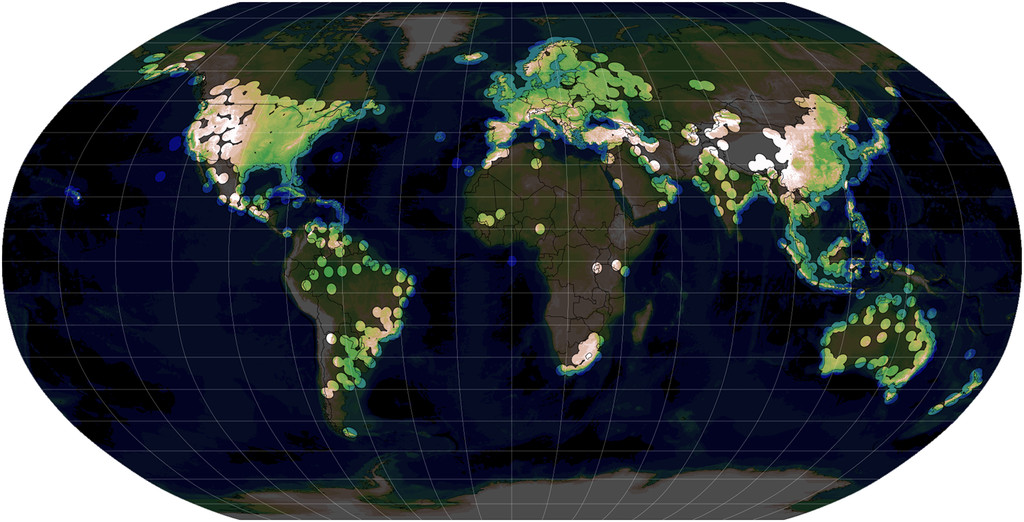
\includegraphics[width=0.96\textwidth,height=0.58\textheight,keepaspectratio]{images/global-weather-radar-coverage-2019.jpg}
\vspace{1mm}
\begin{beamercolorbox}[rounded=true,sep=1ex,wd=\textwidth]{block body}
\scriptsize
\textbf{Source:} Saltikoff et al. (2019), Fig. 1, \emph{Bulletin of the American Meteorological Society}, 100(9), 1739--1752.\hfill
\href{https://doi.org/10.1175/BAMS-D-18-0166.1}{doi:10.1175/BAMS-D-18-0166.1}\par
\textbf{Method:} Estimated radar illumination assumes a 200 km range for every radar; locations are based mainly on the WMO Radar Database (accessed March 2019). The database does not include every operational radar.
\end{beamercolorbox}
\note{Figure 1 from Saltikoff, E., Friedrich, K., Soderholm, J., Lengfeld, K., Nelson, B., Becker, A., Hollmann, R., Urban, B., Heistermann, M., and Tassone, C. (2019), “An Overview of Using Weather Radar for Climatological Studies: Successes, Challenges, and Potential,” Bulletin of the American Meteorological Society, 100(9), 1739--1752, https://doi.org/10.1175/BAMS-D-18-0166.1. The authors used wradlib to map areas illuminated by radar, assuming a 200 km range irrespective of bandwidth, polarization, or local terrain. Most radar locations came from the WMO Radar Database accessed March 2019; the paper notes that not all operational radars are included and describes additional data sources for some countries.}
\end{frame}

\begin{frame}[t]
\slidetitle{Africa's mobile-tower network was growing}
\centering
\begin{tikzpicture}
\begin{axis}[
  width=0.88\textwidth,
  height=0.66\textheight,
  xmin=2009, xmax=2015,
  ymin=100000, ymax=190000,
  xtick={2009,2010,2011,2012,2013,2014,2015},
  xticklabels={2009,2010,2011,2012,2013,2014,2015},
  scaled y ticks=false,
  ytick={100000,120000,140000,160000,180000},
  yticklabels={100000,120000,140000,160000,180000},
  xlabel={Year},
  ylabel={Estimated towers},
  tick label style={font=\scriptsize},
  label style={font=\small},
  axis line style={black!50},
  grid=major,
  major grid style={black!12},
  enlargelimits=false,
  clip=false,
]
\addplot[very thick,MediumRed,mark=*,mark size=2.2pt] coordinates {
  (2009,120000) (2010,125000) (2011,130000) (2012,140000) (2013,150000)
};
\addplot[very thick,MediumRed,dashed,mark=*,mark size=2.2pt] coordinates {
  (2013,150000) (2014,165000) (2015,180000)
};
\node[anchor=south west,font=\small\bfseries,text=DarkBlue,fill=white,inner sep=1pt]
  at (axis cs:2013.5,184000) {$\approx$180 km$^2$ per tower\textsuperscript{*}};
\end{axis}
\end{tikzpicture}

\vspace{-1mm}
{\small TowerXchange estimated 150,000 towers in 2013; its 2015 forecast was 180,000 (dashed).}\par
\vspace{1mm}
{\tiny *Area/count ratio, not coverage: 29.65 million km$^2$ (Africa) $\div$ 165,000 towers (2014 forecast) $\approx$ 180 km$^2$/tower. Area: \href{https://data.un.org/legacy/en/reg/g2.html}{UN Data}.}\par
{\tiny Source: TowerXchange, Issue 10 (October 2014), Fig. 4, “African tower industry achieves launch velocity.”\;
\href{https://www.towerxchange.com/article/2blfxwil8mhol0ggutc00/31-600-or-20-of-africas-towers-are-now-owned-or-operated-by-independent-towercos}{TowerXchange article}.}
\note{Redrawn from TowerXchange Issue 10, October 2014, Figure 4. Historical estimate series: 120,000 (2009), 125,000 (2010), 130,000 (2011), 140,000 (2012), 150,000 (2013). The source marks 2014 (165,000) and 2015 (180,000) as forecasts. Approximate density annotation is calculated as UN Data's Africa surface area (29,648,481 km2) divided by TowerXchange's 2014 forecast (165,000), or about 180 km2 per tower. This is a continent-wide average density, not a tower's service radius or actual coverage. These are historical industry estimates, not current tower counts. Source article: https://www.towerxchange.com/article/2blfxwil8mhol0ggutc00/31-600-or-20-of-africas-towers-are-now-owned-or-operated-by-independent-towercos ; area source: https://data.un.org/legacy/en/reg/g2.html}
\end{frame}

\begin{frame}[t]
\slidetitle{Reconstructing rainfall from cellular links}
\begin{columns}[T,onlytextwidth]
\begin{column}{0.66\textwidth}
\centering
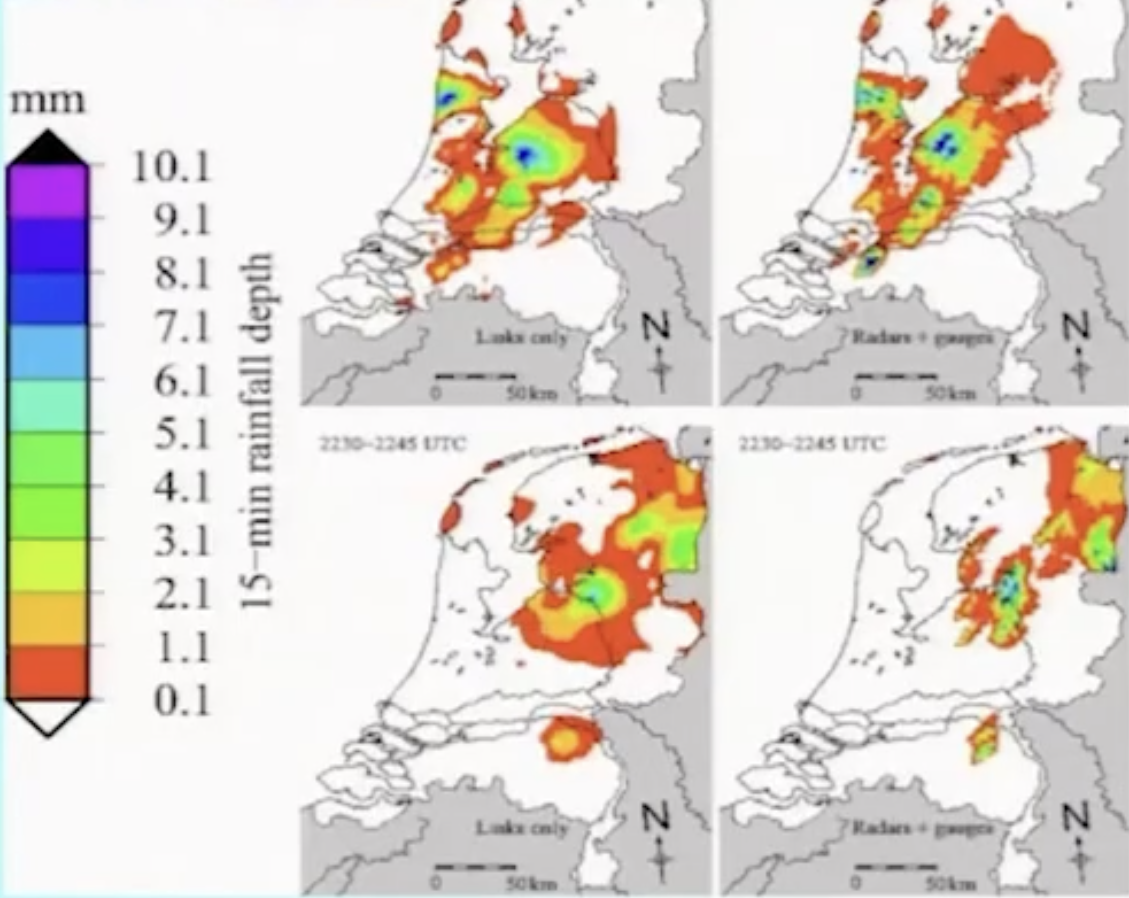
\includegraphics[width=\linewidth,height=0.72\textheight,keepaspectratio]{images/overeem-2013-figure3-crop.png}
\vspace{1mm}
{\scriptsize 15-min rainfall, 10 Sep 2011: 20:30--20:45 UTC (top), 22:30--22:45 (bottom); links (left), radar + gauges (right).}
\end{column}
\begin{column}{0.31\textwidth}
\small
\textbf{Where?} The Netherlands.\par\medskip
\textbf{How?} Convert link attenuation to path-averaged rainfall, then use ordinary kriging from link midpoints to map the field.\par\medskip
\textbf{Comparison?} Link-only estimates are checked against an independent radar-and-gauge product.
\vspace{4mm}
\begin{beamercolorbox}[rounded=true,sep=1ex,wd=\linewidth]{block body}
\footnotesize
\textbf{Source}\par
Overeem, Leijnse, and Uijlenhoet (2013), \emph{PNAS} 110(8), Fig. 3.\par
\href{https://doi.org/10.1073/pnas.1217961110}{doi:10.1073/pnas.1217961110}
\end{beamercolorbox}
\end{column}
\end{columns}
\note{Figure 3, adapted from the original slide screenshot provided by the user, from Overeem, A., Leijnse, H., and Uijlenhoet, R. (2013), “Country-wide rainfall maps from cellular communication networks,” Proceedings of the National Academy of Sciences, 110(8), 2741--2745, https://doi.org/10.1073/pnas.1217961110. The maps show validation cases for 10 September 2011 at 2030--2045 UTC and 2230--2245 UTC. Left panels use commercial microwave links; right panels use radar plus gauges. For each 15-minute period, link rainfall depths are treated as point measurements at the link midpoints and interpolated with ordinary kriging. Radar and gauge data serve as an independent validation comparison, not as inputs to the link-only maps.}
\end{frame}
\end{document}
